
%% Beginning of file 'sample63.tex'
%%
%% Modified 2019 June
%%
%% This is a sample manuscript marked up using the
%% AASTeX v6.3 LaTeX 2e macros.
%%
%% AASTeX is now based on Alexey Vikhlinin's emulateapj.cls 
%% (Copyright 2000-2015).  See the classfile for details.

%% AASTeX requires revtex4-1.cls (http://publish.aps.org/revtex4/) and
%% other external packages (latexsym, graphicx, amssymb, longtable, and epsf).
%% All of these external packages should already be present in the modern TeX 
%% distributions.  If not they can also be obtained at www.ctan.org.

%% The first piece of markup in an AASTeX v6.x document is the \documentclass
%% command. LaTeX will ignore any data that comes before this command. The 
%% documentclass can take an optional argument to modify the output style.
%% The command below calls the preprint style which will produce a tightly 
%% typeset, one-column, single-spaced document.  It is the default and thus
%% does not need to be explicitly stated.
%%
%%
%% using aastex version 6.3
\documentclass[twocolumn]{aastex63}

%% The default is a single spaced, 10 point font, single spaced article.
%% There are five other style options available via an optional argument. 
%% They can be invoked like this:
%%
%% \documentclass[arguments]{aastex63}
%% 
%% where the layout options are:
%%
%%  twocolumn   : two text columns, 10 point font, single spaced article.
%%                This is the most compact and represent the final published
%%                derived PDF copy of the accepted manuscript from the publisher
%%  manuscript  : one text column, 12 point font, double spaced article.
%%  preprint    : one text column, 12 point font, single spaced article.  
%%  preprint2   : two text columns, 12 point font, single spaced article.
%%  modern      : a stylish, single text column, 12 point font, article with
%% 		  wider left and right margins. This uses the Daniel
%% 		  Foreman-Mackey and David Hogg design.
%%  RNAAS       : Preferred style for Research Notes which are by design 
%%                lacking an abstract and brief. DO NOT use \begin{abstract}
%%                and \end{abstract} with this style.
%%
%% Note that you can submit to the AAS Journals in any of these 6 styles.
%%
%% There are other optional arguments one can invoke to allow other stylistic
%% actions. The available options are:
%%
%%   astrosymb    : Loads Astrosymb font and define \astrocommands. 
%%   tighten      : Makes baselineskip slightly smaller, only works with 
%%                  the twocolumn substyle.
%%   times        : uses times font instead of the default
%%   linenumbers  : turn on lineno package.
%%   trackchanges : required to see the revision mark up and print its output
%%   longauthor   : Do not use the more compressed footnote style (default) for 
%%                  the author/collaboration/affiliations. Instead print all
%%                  affiliation information after each name. Creates a much 
%%                  longer author list but may be desirable for short 
%%                  author papers.
%% twocolappendix : make 2 column appendix.
%%   anonymous    : Do not show the authors, affiliations and acknowledgments 
%%                  for dual anonymous review.
%%
%% these can be used in any combination, e.g.
%%
%% \documentclass[twocolumn,linenumbers,trackchanges]{aastex63}
%%
%% AASTeX v6.* now includes \hyperref support. While we have built in specific
%% defaults into the classfile you can manually override them with the
%% \hypersetup command. For example,
%%
%% \hypersetup{linkcolor=red,citecolor=green,filecolor=cyan,urlcolor=magenta}
%%
%% will change the color of the internal links to red, the links to the
%% bibliography to green, the file links to cyan, and the external links to
%% magenta. Additional information on \hyperref options can be found here:
%% https://www.tug.org/applications/hyperref/manual.html#x1-40003
%%
%% Note that in v6.3 "bookmarks" has been changed to "true" in hyperref
%% to improve the accessibility of the compiled pdf file.
%%
%% If you want to create your own macros, you can do so
%% using \newcommand. Your macros should appear before
%% the \begin{document} command.
%%
\newcommand{\vdag}{(v)^\dagger}
\newcommand\aastex{AAS\TeX}
\newcommand\latex{La\TeX}



\usepackage{color}

\usepackage{times}
\newcommand{\sqcm}{cm$^{-2}$}
\newcommand{\alphaox}{$\alpha_{OX}$}
\newcommand{\Gammaxray}{$\Gamma$}

\newcommand{\fek}{Fe~K$\alpha$}
\newcommand{\xmm}{{\em XMM-Newton}}
\newcommand{\nustar}{{\em NuSTAR }}
\newcommand{\chandra}{{\em Chandra}}
\newcommand{\swift}{{\em Swift}}
\newcommand{\suzaku}{{\em Suzaku}}
\newcommand{\sax}{{\em BeppoSAX}}
\usepackage[space]{grffile}
\usepackage[]{amsmath}
\usepackage{amssymb}
\usepackage[normalem]{ulem}
\usepackage{natbib}
\usepackage{longtable}
%\usepackage{hyperref}
\usepackage{comment}
\bibpunct{(}{)}{;}{a}{}{,}
%\usepackage{pdflscape}	% Landscape pages
\usepackage{amsmath} % or simply amstext
\newcommand{\angstrom}{\text{\normalfont\AA}}
\usepackage{url}
\texorpdfstring
%\usepackage{showframe}









%% Reintroduced the \received and \accepted commands from AASTeX v5.2
\received{November  X, 2019}
\revised{November  X, 2019}
\accepted{\today}
%% Command to document which AAS Journal the manuscript was submitted to.
%% Adds "Submitted to " the argument.
\submitjournal{APJ}

%% For manuscript that include authors in collaborations, AASTeX v6.3
%% builds on the \collaboration command to allow greater freedom to 
%% keep the traditional author+affiliation information but only show
%% subsets. The \collaboration command now must appear AFTER the group
%% of authors in the collaboration and it takes TWO arguments. The last
%% is still the collaboration identifier. The text given in this
%% argument is what will be shown in the manuscript. The first argument
%% is the number of author above the \collaboration command to show with
%% the collaboration text. If there are authors that are not part of any
%% collaboration the \nocollaboration command is used. This command takes
%% one argument which is also the number of authors above to show. A
%% dashed line is shown to indicate no collaboration. This example manuscript
%% shows how these commands work to display specific set of authors 
%% on the front page.
%%
%% For manuscript without any need to use \collaboration the 
%% \AuthorCollaborationLimit command from v6.2 can still be used to 
%% show a subset of authors.
%
%\AuthorCollaborationLimit=2
%
%% will only show Schwarz & Muench on the front page of the manuscript
%% (assuming the \collaboration and \nocollaboration commands are
%% commented out).
%%
%% Note that all of the author will be shown in the published article.
%% This feature is meant to be used prior to acceptance to make the
%% front end of a long author article more manageable. Please do not use
%% this functionality for manuscripts with less than 20 authors. Conversely,
%% please do use this when the number of authors exceeds 40.
%%
%% Use \allauthors at the manuscript end to show the full author list.
%% This command should only be used with \AuthorCollaborationLimit is used.

%% The following command can be used to set the latex table counters.  It
%% is needed in this document because it uses a mix of latex tabular and
%% AASTeX deluxetables.  In general it should not be needed.
%\setcounter{table}{1}

%%%%%%%%%%%%%%%%%%%%%%%%%%%%%%%%%%%%%%%%%%%%%%%%%%%%%%%%%%%%%%%%%%%%%%%%%%%%%%%%
%%
%% The following section outlines numerous optional output that
%% can be displayed in the front matter or as running meta-data.
%%
%% If you wish, you may supply running head information, although
%% this information may be modified by the editorial offices.
\shorttitle{Mrk 1018}
\shortauthors{Bing Lyu et al.}
%%
%% You can add a light gray and diagonal water-mark to the first page 
%% with this command:
%% \watermark{text}
%% where "text", e.g. DRAFT, is the text to appear.  If the text is 
%% long you can control the water-mark size with:
%% \setwatermarkfontsize{dimension}
%% where dimension is any recognized LaTeX dimension, e.g. pt, in, etc.
%%
%%%%%%%%%%%%%%%%%%%%%%%%%%%%%%%%%%%%%%%%%%%%%%%%%%%%%%%%%%%%%%%%%%%%%%%%%%%%%%%%
\graphicspath{{./}{figures/}}
\graphicspath{{./}{pic/}}
%% This is the end of the preamble.  Indicate the beginning of the
%% manuscript itself with \begin{document}.

\begin{document}

\def\sectionautorefname{Section}
\def\subsectionautorefname{Section}

\title{Long term multi-wavelength evolution of a Changing-Look AGN: Mrk~1018}

%% LaTeX will automatically break titles if they run longer than
%% one line. However, you may use \\ to force a line break if
%% you desire. In v6.3 you can include a footnote in the title.

%% A significant change from earlier AASTEX versions is in the structure for 
%% calling author and affiliations. The change was necessary to implement 
%% auto-indexing of affiliations which prior was a manual process that could 
%% easily be tedious in large author manuscripts.
%%
%% The \author command is the same as before except it now takes an optional
%% argument which is the 16 digit ORCID. The syntax is:
%% \author[xxxx-xxxx-xxxx-xxxx]{Author Name}
%%
%% This will hyperlink the author name to the author's ORCID page. Note that
%% during compilation, LaTeX will do some limited checking of the format of
%% the ID to make sure it is valid. If the "orcid-ID.png" image file is 
%% present or in the LaTeX pathway, the OrcID icon will appear next to
%% the authors name.
%%
%% Use \affiliation for affiliation information. The old \affil is now aliased
%% to \affiliation. AASTeX v6.3 will automatically index these in the header.
%% When a duplicate is found its index will be the same as its previous entry.
%%
%% Note that \altaffilmark and \altaffiltext have been removed and thus 
%% can not be used to document secondary affiliations. If they are used latex
%% will issue a specific error message and quit. Please use multiple 
%% \affiliation calls for to document more than one affiliation.
%%
%% The new \altaffiliation can be used to indicate some secondary information
%% such as fellowships. This command produces a non-numeric footnote that is
%% set away from the numeric \affiliation footnotes.  NOTE that if an
%% \altaffiliation command is used it must come BEFORE the \affiliation call,
%% right after the \author command, in order to place the footnotes in
%% the proper location.
%%
%% Use \email to set provide email addresses. Each \email will appear on its
%% own line so you can put multiple email address in one \email call. A new
%% \correspondingauthor command is available in V6.3 to identify the
%% corresponding author of the manuscript. It is the author's responsibility
%% to make sure this name is also in the author list.
%%
%% While authors can be grouped inside the same \author and \affiliation
%% commands it is better to have a single author for each. This allows for
%% one to exploit all the new benefits and should make book-keeping easier.
%%
%% If done correctly the peer review system will be able to
%% automatically put the author and affiliation information from the manuscript
%% and save the corresponding author the trouble of entering it by hand.


\author{To be determind}

\begin{comment}
\author[0000-0001-8879-368X]{Bing Lyu}
\affiliation{Huazhong University of Science and Technology \\
School of Physics, 1037 Luoyu Road \\
Wuhan, 430074, China \\}
%\affil{Shanghai Astronomical Observatory\\ CAS, Nandan Road 80 \\ Shanghai, 200030, China}
%\nocollaboration
\author[0000-0002-5385-9586]{Zhen Yan}
\affil{Shanghai Astronomical Observatory\\
CAS, Nandan Road 80 \\
Shanghai, 200030, China}



\author[0000-0002-3844-9677]{Wenfei Yu}
\affiliation{Shanghai Astronomical Observatory\\
CAS, Nandan Road 80 \\
Shanghai, 200030, China}
%\collaboration{(AAS Journals Data Scientists collaboration)}

\author[0000-0003-4773-4987]{Qingwen Wu}
\affiliation{Huazhong University of Science and Technology \\
School of Physics, 1037 Luoyu Road \\
Wuhan, 430074, China \\}

%\correspondingauthor{Qingwen Wu}
%\email{qwwu@hust.edu.cn}
\end{comment}
%\nocollaboration



%% Note that the \and command from previous versions of AASTeX is now
%% depreciated in this version as it is no longer necessary. AASTeX 
%% automatically takes care of all commas and "and"s between authors names.

%% AASTeX 6.3 has the new \collaboration and \nocollaboration commands to
%% provide the collaboration status of a group of authors. These commands 
%% can be used either before or after the list of corresponding authors. The
%% argument for \collaboration is the collaboration identifier. Authors are
%% encouraged to surround collaboration identifiers with ()s. The 
%% \nocollaboration command takes no argument and exists to indicate that
%% the nearby authors are not part of surrounding collaborations.

%% Mark off the abstract in the ``abstract'' environment. 
\begin{abstract}
We present multi-wavelength and long-term evolution of a Changing-Look active galactic nucleus (CL AGN), Mrk~1018. Before fading into the faint state, it shows rapid variability in X-ray and optical band. While Mrk~1018 shows strong correlation between UVOT and X-ray band, the flux in UVOT varies more than that in X-ray as a whole but reverses during type transition within short timescale. The type transition timescale for Mrk~1018 is around 2 years(between 2013--2015) or less, while the minimum timescale for variability can be as short as $\sim$ 100 days during transition state and several days in the faint state. The photon index($\Gamma$) indicating the hardness in X-ray and $\alpha_{OX}$ representing the relative strength of ultraviolet to X-ray, both appear as ``V-shape'' compared to luminosity. We find that $\alpha_{OX}-L_{UV}$ diagram is well linked to type of Mrk~1018 in comparison with another two CL AGNs. However, only weak variability appears in the radio band, might infer different radiation efficiency of accretion process.  
\end{abstract}
%% Keywords should appear after the \end{abstract} command. 
%% See the online documentation for the full list of available subject
%% keywords and the rules for their use.
\keywords{galaxies: active – galaxies: individual: Mrk 1018 – galaxies: Seyfert}



%% From the front matter, we move on to the body of the paper.
%% Sections are demarcated by \section and \subsection, respectively.
%% Observe the use of the LaTeX \label
%% command after the \subsection to give a symbolic KEY to the
%% subsection for cross-referencing in a \ref command.
%% You can use LaTeX's \ref and \label commands to keep track of
%% cross-references to sections, equations, tables, and figures.
%% That way, if you change the order of any elements, LaTeX will
%% automatically renumber them.
%%
%% We recommend that authors also use the natbib \citep
%% and \citet commands to identify citations.  The citations are
%% tied to the reference list via symbolic KEYs. The KEY corresponds
%% to the KEY in the \bibitem in the reference list below. 

\section{Introduction}\label{sec:intro} 

The bright nuclei of many galaxies called active galactic nuclei (AGNs) are more luminous at the central region than the remaining area. The first class of AGNs showing emission lines are found by Carl Seyfert after whom these AGNs are now named. Based on the optical spectral emission line, these galaxies are classfied as Type I/II AGNs. Type I Seyfert (S1) galaxies, show broad lines, allow lines and narrower forbidden lines, while Type II Seyfert (S2) galaxies show only both permitted and forbidden narrow lines. Sub-classes (e.g. Seyfert 1.5, 1.8 and 1.9) are introduced by \citet{1976MNRAS.176P..61O,1981ApJ...249..462O} based on the width and relative flux of broad-line components to the narrow-line component. For a Seyfert 1.9, it is a Seyfert 1 where only $H\alpha$ line appears in the broad-line components. 

In the unification model, AGNs are believed to be powered by the accretion of a central supermassive black hole with torus surrounded, and the different types are explained as the effect of different inclinations relative to the line of sight \citep[see][]{1993ARA&A..31..473A}. Under this model, Type 1 AGNs are face-on to observer with broad line visible to us, while Type 2 AGNs are edge-on with broad emission line blocked by surrounding torus.

%\textcolor{red}

{However, more and more AGNs, have been discovered to change their source classification (so called Changing-Look AGNs) within timescale of years or decades \citep[e.g.][]{2016MNRAS.457..389M, 2016ApJ...826..188R, 2018ApJ...864...27S, 2019ApJ...874....8M,2020MNRAS.491.4925G}, 
%{MacLeod2016,Ruan2016,Stern2018,MacLeod2019,Graham2020}
which show the disappearance/appearance of broad emission lines \citep[e.g.][]{2016MNRAS.457..389M,?}. Many of them also show dramatic flux variability in optical/ultraviolet and/or X-ray \citep[e.g.][]{2017ApJ...846L...7S,?}. According to the traditional AGN unification model, the type changes should be related with the obscuration by the torus. However, some evidence show that the type transition are driven by the activity of the AGN. For example, it is found that there is no intrinsic absorption of X-ray spectrum for some CL-AGNs. Besides, the large variability in mid-infrared band for some CL-AGNs\citep[e.g.][]{2017ApJ...846L...7S} does not support the varying obscuration scernario. The optical and X-ray light curve in good correlation might also support the activity of the central engine. Thus, the multi-wavelength observations are very import tool to study the activities of the central engine. Since the emission of different wavelengths are from different components or different radiative mechanism. %For example, the X-ray emission is from the corona, the optical/UV emission is from accretion disk and the radio emission is from jet. 
Therefore, investigating the multi-wavelength evolution will reveal the links between changing-look behavior and the different components and provide a clue about the changing-look mechanism.}

%The discussion about whether the type transition on such short timescale is related to activeness of central engine or obscuration event is still continuing. 

%emphasize the importance of multi-wavelength evolution, then introduce the observations in different bands reported previously.


Mrk~1018 at $z=0.042436$ is known to be a Changing-Look AGN, which has undergone a full cycle with twice type transition. \citet{1986ApJ...311..135C} reports that the type of Mrk~1018 transits from S1.9 to S1 between 1979 and 1984. \citet{2016A&A...593L...8M} reports that Mrk~1018 returns to S1.9 between around 2013 and 2015 after 30 years as a S1 \citep[see also][]{2017A&A...607L...9K}. %A tidal eruption event could not account for the Mrk 1018's type change. 
Observations in different wavelengths have covered the time before and after the changing-look event. %...... (补充不同波段观测信息)
As reported in \citet{2016A&A...593L...9H}, during 2010-2016, the optical continuum brightness and X-ray flux drops by a factor of $\sim$ 17 and $\sim 8$, respectively, with no intrinsic absorption in the X-ray spectrum detected. So it's a good target to explore the intrinsic mechanism of type transition of CL AGNs through the multi-wavelength evolution.

%An explanation of obscuration event for the variability is ruled out, since no intrinsic absorption in the X-ray spectrum is detected. It comes to the conclusion that change of type is consistent with declining accretion rate. \citet{2017A&A...607L...9K} reported the mini-outburst of Mrk~1018 in October 2016 with the brightening by a factor of 1.9 at least to February 2017. Far-UV continuum flux also increased by a factor of 1.5 in around one year during the outburst. It seems that radiation of corona and accretion disk comes from near region. We notice that Mrk~1018 has also experienced the re-brightening during the types transition period simultaneously in X-ray and UVOT band by a factor of $\sim3$ and $\sim1.3$, respectively, between 2013 Mar and 2013 Jun. With broad-band spectrum fitting in two states, \citet{2018MNRAS.480.3898N} suggests the drop of soft X-ray excess contributing most ionizing photons causes the disappearance of Broad Line Region(BLR) then the type transition. \citet{2018ApJ...861...51K} models the broad-line component with a recoiled super-massive black hole scenario with a $\sim$29 years orbital period and predicts that if the type transition repeats as past, it would occur again in mid-2020s. Before that, what the mechanism for such short-timescale light curve variability for AGN and type transition is remains unclear. 

In this work, we perform an extensive data analysis to study the luminosity and spectral evolution of Mrk~1018 at X-ray, optical/ultraviolet and radio bands. This paper is structured as followings: In \autoref{sec:data}, we describe the observations and data reduction in X-ray, optical/ultraviolet and radio bands. In \autoref{sec:result}, we present multi-wavelength observation results. In \autoref{sec:discussion}, we discuss possible explanations for the observation of Mrk~1018. Hereafter, we adopt $H_0$=70 km s$^{-1}$ Mpc $^{-1}$, $\Omega_{m}$=0.3, and $\Omega_{\Lambda}=0.7 $ as cosmological parameters, luminosity distance at 187 Mpc and the latest black hole (BH) mass measurement $\log(M_{\rm{BH}}/M_{\odot})=7.84$ \citep{2017MNRAS.472.3492E,2018MNRAS.480.3898N}. 
%\clearpage


\section{Data Analysis}\label{sec:data}
\subsection{X-ray}
We analyse all the public archival data of \swift, \xmm, \chandra and \nustar during 2005--2018. During the X-ray spectral fitting, the column density $n_{\rm{H}}$ is fixed at 0.0243 $\times 10^{22}$ cm$^{-2}$ since the intrinsic absorption is negligible \citep[see ][]{2016A&A...593L...9H}. The 2--10~keV fluxes are calculated by {\it cflux} component within {\scriptsize XSPEC} (v12.10). All the X-ray observation information and best fit parameters including photon index ($\Gamma$, hereafter), unabsorbed flux in 2--10~keV ($F_{\rm{2-10~keV}}$) are listed in \autoref{tab:table1}. The long term X-ray light curve in 2--10~keV is shown in \autoref{fig:multi-lc-secondaxis}.
%and \autoref{fig:x-ray-lc-rp-secondaxis}.


\subsubsection{\swift/XRT}
The X-Ray Telescope (XRT) on board the \swift satellite has the most frequent X-ray observations of Mrk~1018. We process all the archive data of \swift/XRT observations performed in photon counting mode with {\scriptsize XRTPIPELINE}\footnote{\url{http://swift.asdc.asi.it}}. The source region is a circle centered at the nucleus of Mrk 1018, the radius of which is determined by the count rate of each observation according to \citet{2009MNRAS.397.1177E}. We use {\scriptsize XSELECT} to extract the source and background spectra. When the counts of an XRT spectrum is less than 200, we use C-stat method for fitting with minimum one count per bin. Otherwise, the spectrum is grouped by minimum of 20 counts per bin and fitted with Chi-stat method. All the XRT spectra of Mrk~1018 in 0.5--10~keV range are fitted with an absorbed power-law model. 


\subsubsection{\chandra/ACIS-S}
There are 6 Chandra observations released in archive. We extract all the ACIS-S spectra with CIAO (v4.10) \footnote{\url{http://cxc.harvard.edu/ciao/threads/index.html}} and {\scriptsize CALDB} (v4.1). The selection of source and background regions follows \citet{2017ApJ...840...11L}. For observation in 2010 (ObsID 12868), the pile-up effect should be carefully taken into account. We notice that different treatments on the pile-up effect are adopted \citep[see ][]{2017ApJ...840...11L,2016A&A...593L...9H,2017A&A...607L...9K}. Here we exclude the brightest 9 pixels following \citet{2016A&A...593L...9H} for this observation. Then all the spectra in 0.5--10~keV range are grouped by minimum of 20 counts per bin and fitted with an absorbed power-law plus a gaussian component. 

%For this observation, the selection of source and background regions  are followed \citet{2017ApJ...840...11L}.  takes into account the pile-up effect with a JDPILEUP component and get the  $\Gamma =1.97_{+0.04}^{-0.03}$. It's similar to our result $\Gamma =2.02\pm{0.03}$ when we adopt the same pile-up model. \citet{2016A&A...593L...9H} excluded the brightest 9 pixels to avoid pile-up effects and get a lower $\Gamma =1.68\pm0.04$ determined from 4-8 keV range spectrum. The correction for pile-up effects will make the spectrum softer. \citet{2017A&A...607L...9K} ignored the pile-up effects and get a similar $\Gamma =1.7\pm0.03$ fitting in 0.5-8 keV. The fitting range selection will also influence the parameter $\Gamma$. So we adopt values from \citet{2017A&A...607L...9K} for the observation in 2010(MJD 55527).

\subsubsection{\xmm/EPIC-PN}
Only 2 observations from \xmm have been released, which are in 2005 (ObsID 201090201) and 2008 (ObsID 554920301), respectively. We reprocess the PN data with {\scriptsize EPPROC} in SAS-16.1.0.\footnote{\url{https://www.cosmos.esa.int/web/xmm-newton}}. The spectrum is grouped by minimum of 30 counts per bin and fitted in the 2--10~keV range based on an absorbed power-law model. 



\subsubsection{\nustar}
There are 5 public observations of \nustar in the archive, which are processed through the {\scriptsize NUPIPELINE} task of the {\scriptsize NUSTARDAS} package. The source region is a 50-arcsec-radius circle at the center of AGN, and background is extracted from region off source. The spectrum is grouped by minimum of 30 counts per bin and fitted in the 3--79~keV range with an absorbed power-law model.


\subsection{Optical/ultraviolet}
\subsubsection{\swift/UVOT}
There are six filters in optical/ultraviolet band of \swift/UVOT: V,B,U,UVW1,UVM2 and UVW2. We use the tool \textit{uvotsource} to do the aperture photometry for each filter of all the observations. The source aperture radius is 5$\arcsec$ and the background is chosen in a blank region with much larger aperture radius. The UVOT fluxes are corrected for the Galactic extinction with \texorpdfstring{E(B$-V$) = 0.03645} \citet{2018MNRAS.480.3898N} and $R_{V}=3.1$. Then we calculate  $A_{\lambda}$ by using extinction curve from \citet{2007ApJ...663..320F} for U, UVW1, UVM2, and 
UVW2 band as 0.31, 0.35, 0.25, and 0.18, respectively. 

According to the spectrum of the host galaxy of Mrk 1018 in \citep{2018MNRAS.480.3898N}, we discard all the results of V and B bands since the emission of which are dominated by the host galaxy even in the bright phase. We also find that the emission from the nucleus at other filters are similar to or less than the host galaxy after 2016 \citep{2018MNRAS.480.3898N}, which is consistent with that the UV flux become nearly constant after 2016 (see \autoref{fig:multi-lc-secondaxis}). 



%f_uw2=(constants.c/(1928*units.AA)).to(u.Hz).value
%f_um2=(constants.c/(2246*units.AA)).to(u.Hz).value
%f_uw1=(constants.c/(2600*units.AA)).to(u.Hz).value
%f_uuu=(constants.c/(3465*units.AA)).to(u.Hz).value



%The Galactic extinction correction with \texorpdfstring{E(B$-V$) = 0.024}. mag \footnote{Retrieved via the NASA/IPAC Extragalactic Database (NED): \url{http://ned.ipac.caltech.edu/}} with extinction model from \citet{2007ApJ...663..320F} is adopted.  
%($A_V=$ 0.075 and $R_{V}=3.1$)


\subsection{Radio}
%\label{subsec:vla}
%\subsubsection{VLA}
We search all the historical VLA observations on Mrk~1018 within the field of view. We analyse the data with CASA version 5.3.0\citep{2007ASPC..376..127M}. For data reduction of the old VLA data (project AU0020, AB0476, AB0540 and AB0878), we manually flag and calibrate the data, then clean the image following the instruction\footnote{\url{https://casaguides.nrao.edu/index.php/VLA_5_GHz_continuum_survey_of_Seyfert_galaxies}}. For all the JVLA data(project 16A-444, 16B-084), calibrations are performed using script EVLA\_pipeline1.4.2\footnote{\url{https://science.nrao.edu/facilities/vla/data-processing/pipeline/scripted-pipeline}}. Different bands are split into different MS files after pipeline calibration and RFI check. Then the source is imaged using TCLEAN method and flux is estimated via IMFIT task. The flux density uncertainty is calculated as $\sigma_{S}=\sqrt{(rms)^2+(0.05\times S)^2}$, where $5\%$ absolute flux error is taken into account. Radio spectral index $\alpha$ is estimated following $S_v \propto v^{-\alpha}$. Results and survey data in FIRST\citep{1994ASPC...61..165B,1995ApJ...450..559B} and Stripe 82\citep{2011AJ....142....3H} from archival papers are listed in Table.~\ref{tab:tableradio}.

\section{Results}
\label{sec:result}

\subsection{Multi-band light curve}

\begin{figure*}
\centering
	% To include a figure from a file named example.*
	% Allowable file formats are eps or ps if compiling using latex
	% or pdf, png, jpg if compiling using pdflatex
	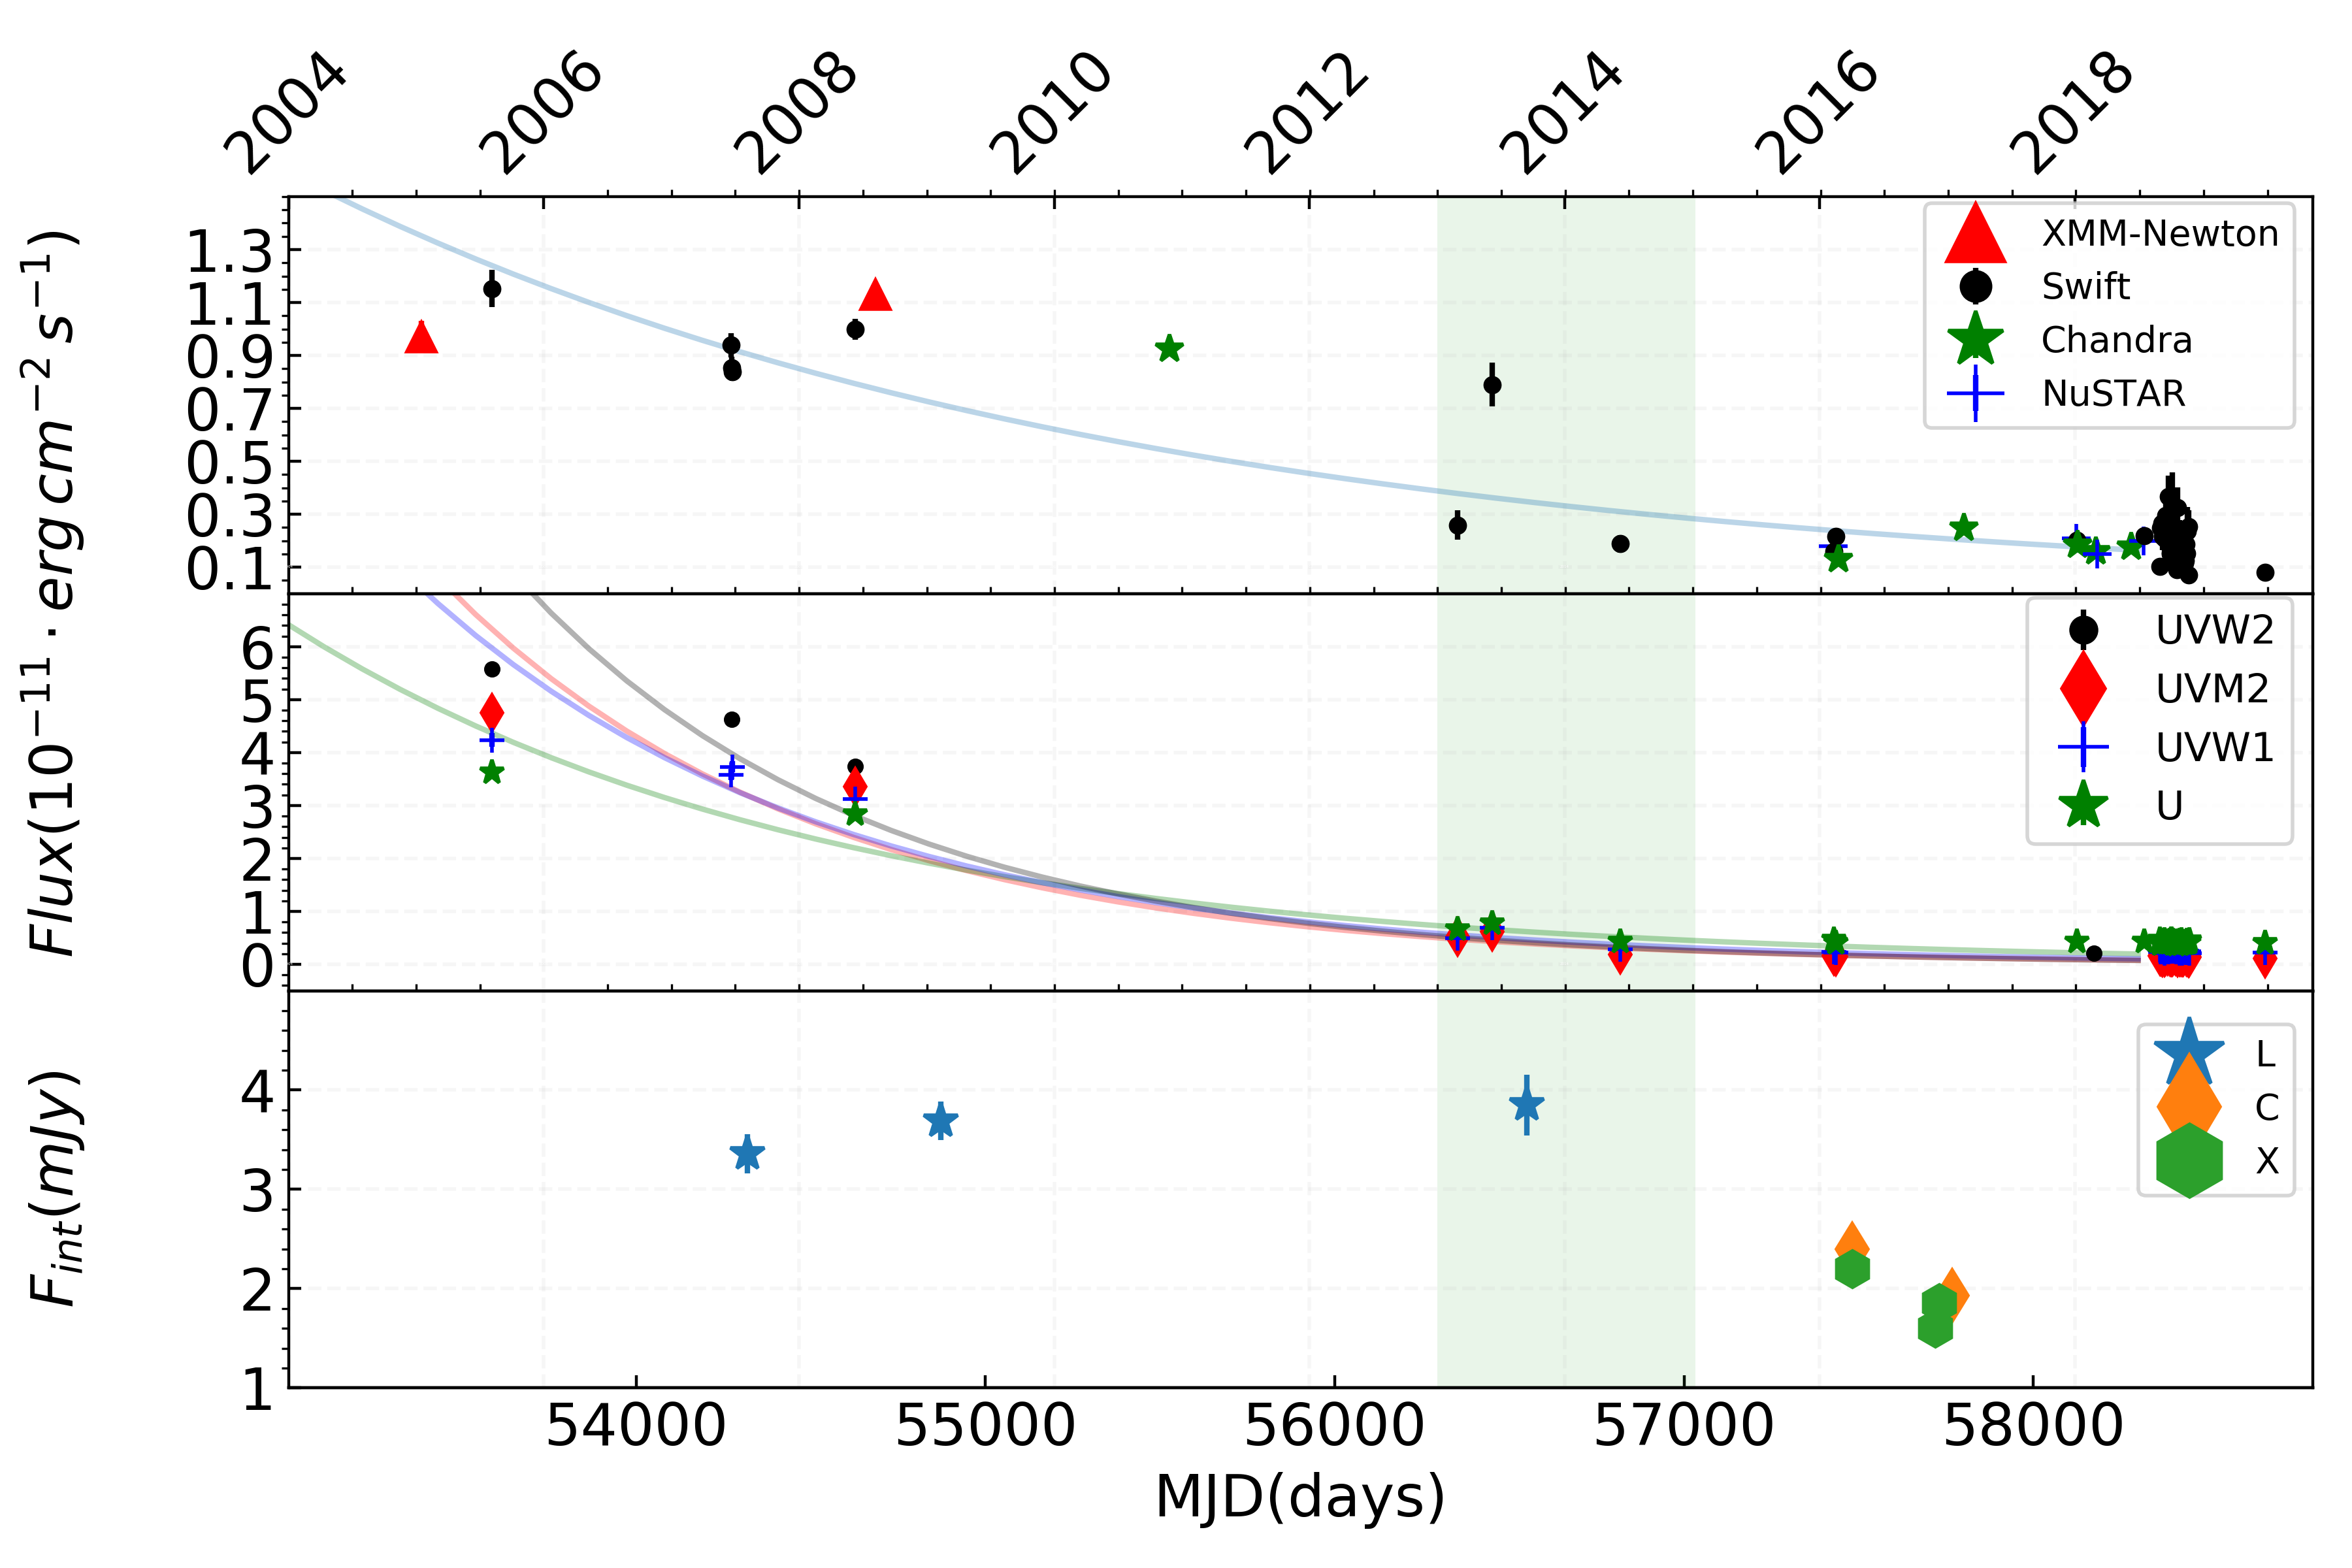
\includegraphics[width=\textwidth]{./pic/subplots-xrt_uvot-radio-second.png}
    \caption{Multi-wavelength light curve of Mrk~1018. Lines shows the fit of light curve with $F=S_0 e^{-(t-t_0)/\tau }$ in X-ray and UVOT band during the main decay phase around 2005--2016. Green shallow shows the inferred transition phase between 2013--2015.  While in faint state after 2016, there is still rapid variability in X-ray, see also \autoref{fig:x-ray-lc-rp-secondaxis} for details and optical radiation is dominated by host galaxy.}
    \label{fig:multi-lc-secondaxis}
\end{figure*}

\begin{figure*}
\centering
	% To include a figure from a file named example.*
	% Allowable file formats are eps or ps if compiling using latex
	% or pdf, png, jpg if compiling using pdflatex
	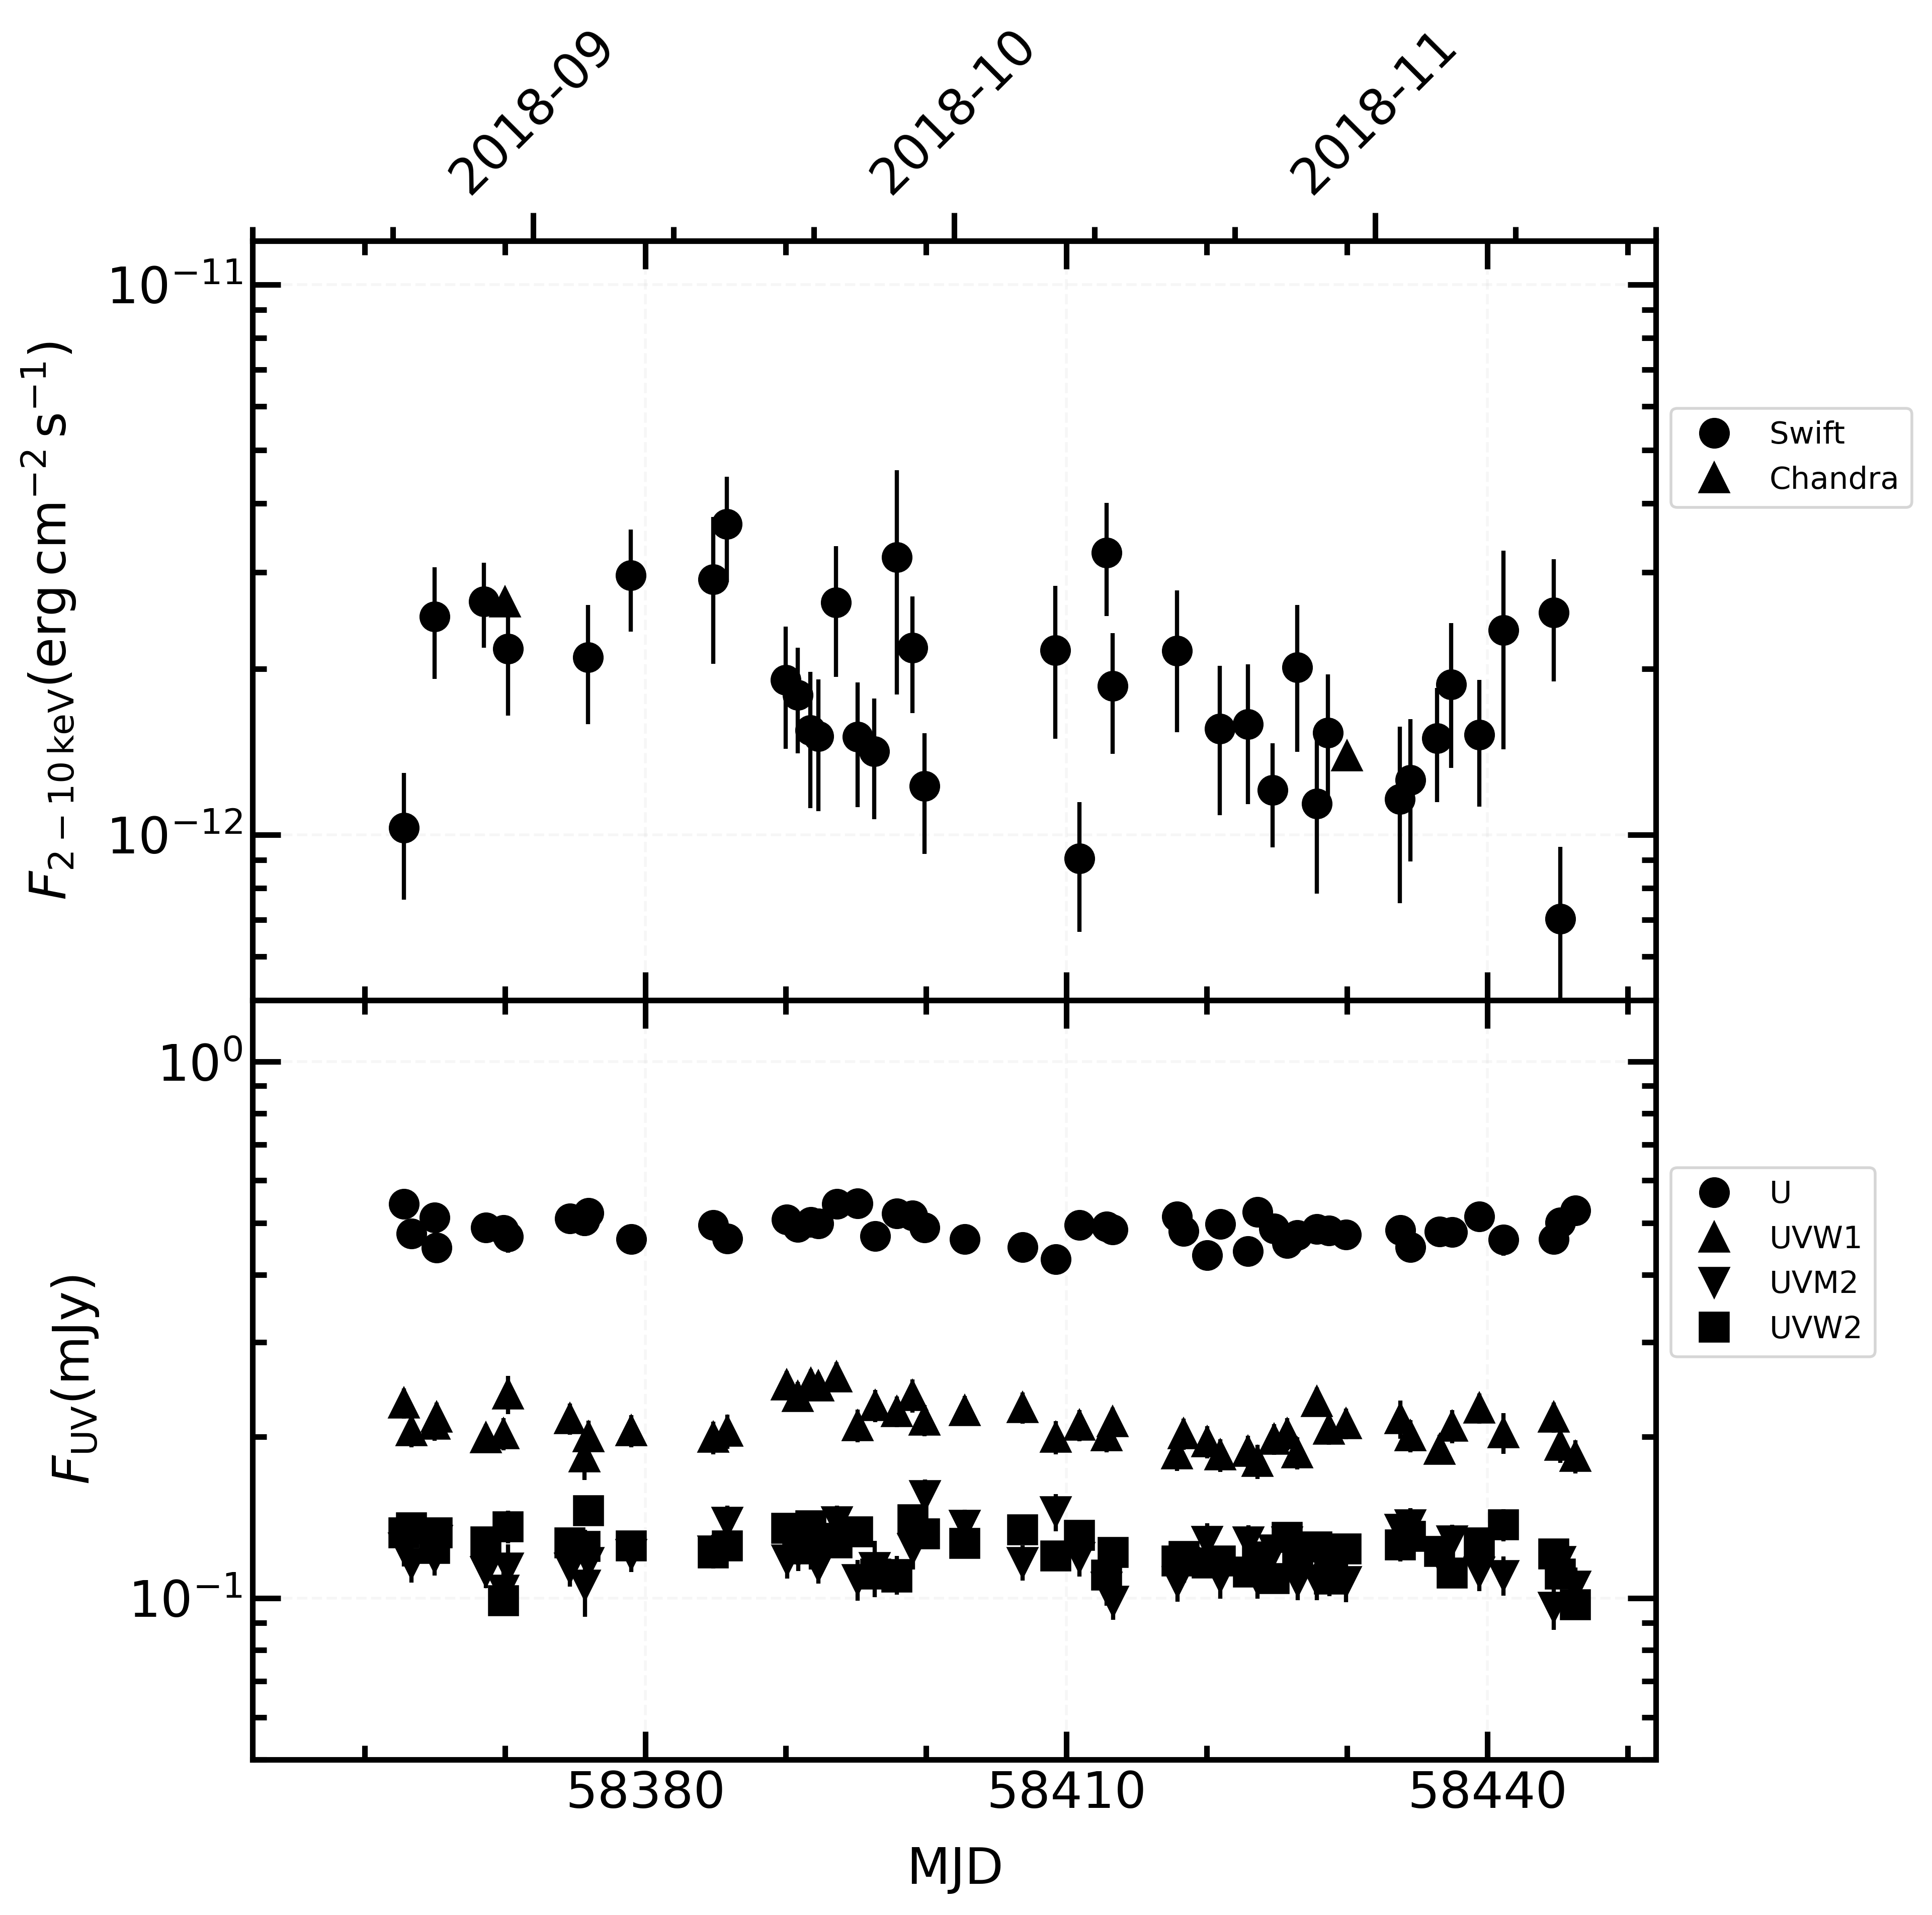
\includegraphics[width=0.8\textwidth]{./pic/subplots-xrt_uvot-radio-second-right-part.png}
    \caption{Light curve of Mrk~1018 in X-ray based on the \swift data after MJD 58350. Mrk~1018 shows rapid variability with $\sigma^2_{rms} = 0.047 \pm 0.0045 $. Variability can reach a factor of $\sim3$ within 30 days.}
    \label{fig:x-ray-lc-rp-secondaxis}
\end{figure*}


Multi-band light curve of Mrk~1018 is shown in \autoref{fig:multi-lc-secondaxis}. During the main decay phase($\sim 2004-2016$), brightness in X-ray and UVOT band drops by a factor $\sim20$ and $\sim9$ in 12 years. During the transition phase($\sim 2013-2015$), we find that brightness in X-ray and UVOT band increases by a factor $\sim3.2$ and $\sim1.4$ in 100 days and then drops by a factor $\sim4.2$ and $\sim2.5$ in 400 days. X-ray flux shows strong correlation with UVOT data during the main decay phase. The spearmanr coefficiency between simultaneous flux of xrt and four uvot band(uvm2,u,uvw1,and uvw2) are 0.99, 0.9, 0.86, 0.94, respectively. We find an outlier in \autoref{fig:correlation-uvot-xray} since the flux during this period in x-ray and four uvot band(uvm2,u,uvw1,and uvw2) increases by a factor of $\sim 3.2$ and $\sim 1.2$, $\sim 1.2$, $\sim 1.4$, $\sim 1.5$, respectively, from MJD 56352 to 56450. Then the flux fades by a factor of $\sim 4.2$ and $\sim 3.3$, $\sim 1.8$, $\sim 2.5$, $\sim 3$, respectively, from MJD 56450 to 56817. The slopes between log($F_{2-10keV}$) and four band log($\lambda F_{\lambda}$) are 1.7, 1.1, 1.5, 1.8, respectively, after excluding the outlier. Mrk~1018 shows rapid variability in X-ray within days with a factor of $\sim3$ when it is in faint state (after 2016) (see \autoref{fig:x-ray-lc-rp-secondaxis}). Root Mean Square($\sigma^2_{rms} = 0.047 \pm 0.026 $) of X-ray light curve in faint state is estimated according to \citet{1999ApJ...524..667T}. Flux in radio band decreases by 20 percent from MJD 57481 to MJD 57719 after the type transition, while the whole light curve shows only weak variability by a factor of less than 2.

\begin{comment}
is calculated with  
\begin{equation}
\sigma^2_{rms}=\frac{1}{N\mu^2}\sum_{i=1}^{N}[(X_i-\mu)^2-\sigma_i^2]
\end{equation}
The error on $\sigma^2_{rms}$ is $s_D/(\mu^2\sqrt{N})$, where \begin{equation}
s_D^2=\frac{1}{N-1}\sum_{i=1}^{N}\{[(X_i-\mu)^2-\sigma_i^2]-\sigma^2_{rms}\mu^2\}^2
\end{equation}
\end{comment}



 The luminosity of Mrk 1018 starts to decline after a 30-years plateau phase \citep[see][]{2016A&A...593L...8M}. In order to roughly estimate the characteristic decay timescale, we then use an exponential function ($F=S_0\,e^{-(t-t_0)/\tau }$) to fit the X-ray (MJD 53385-58317) and optical/UV (MJD 53587-56818) light curves \footnote{Since the fluxes of the six filters of UVOT are all dominated by the host galaxy after $\sim$ MJD 57429. }. The characteristic decay timescale $\tau$ is obtained as $\sim$2340, $\sim$1510, 1160, 1060, and 1010 days for light curve in X-ray, U, UVW1, UVM2, UVW2 band. 
 



\subsection{SED between X-ray and ultraviolet}\label{subsec:xray-uvot-sed}
As the flux drops in X-ray and UVOT band, the spectrum also changes, and the temperature of disk declines as well, see \autoref{fig:xray-uvot-sed}.





%Instruments indicate by C-\chandra, S-\swift, X-\xmm, N-\nustar.








\subsection{Evolution of ~\texorpdfstring{$\Gamma$}. and ~\texorpdfstring{$\alpha_{OX}$}.~ with Eddington rate \label{subsec:g-f}}
We use the $\Gamma$ in X-ray and \alphaox ~ as probe to trace the relationship between corona and accretion disk during the type transition of Mrk~1018. Here we define \alphaox as :
%\begin{equation}
%\alpha_{OX}  = - \frac{\log(\lambda F_{2600 \angstrom}/\nu F_{2keV})}{\log(\nu_{ 2600 \angstrom }/\nu_{2keV})}+1
%\end{equation}
\begin{equation}
\alpha_{OX} = \frac{\log (L_\mathrm{UV} / L_\mathrm{X} )} {\log (\nu_\mathrm{X} /  \nu_\mathrm{UV} )}\label{definition_alpha_ox}
\end{equation}
, where the $L_\mathrm{UV}$ is from the UVW1 filter with central wavelength {2600{$\angstrom$}} and full-width at half max of $\sim 683\angstrom$ \citep{2008MNRAS.383..627P} and the $L_\mathrm{X}$ is the luminosity at 2 keV, which are consistent with previous literature. Only data before 2014 (2016???) is used for estimation of $\alpha_{OX}$. Based on all X-ray spectrum fit, we present the photon index evolution with flux and Eddington rate, as shown in \autoref{fig:xrayappendgood-fandg-tmap}. For XRT observations, we only adopt data with 0.7$\le \chi^2_{reduced} \le$1.5. The $\Gamma$ vs Eddington rate diagram shows distinct anti-positive/positive correlation when $L_{2-10~ keV}/L_{Edd}$ below/above the so-called critical Eddington rate around 0.002$\sim$ 0.01. However, we find that it transits in two branches in short timescale(100-800 days). We emphasise that Mrk~1018 increases its flux in X-ray by a factor $\sim3$ from MJD 56352 to 56450, while $\Gamma$ drops from $\sim1.8$ to $\sim1.4$, which appeares in two branches. However, the $\alpha_{OX}$ varies just a little and appears in left branch during the same time. The $\alpha_{OX}$-Eddington rate diagram is in good agreement with two other changing-look AGNs, see \autoref{fig:alpha_ox_luv}. 

According to \autoref{definition_alpha_ox}, if $ L_\mathrm{X} \propto (L_\mathrm{UV})^{a}$, we derive that $\alpha_{OX}\propto (\frac{1}{a}-1) \log L_\mathrm{X}$, and $\alpha_{OX}\propto (1-a) \log L_\mathrm{UV}$.



\subsection{Correlation between X-ray and radio}\label{subsec:xray-radio}
We adopt data from intervals between X-ray and radio band as short as possible to explore the quasi-simultaneous flux in two bands. The correlation between the radio and X-ray flux is weak with a spearmanr coefficiency: -0.54, since the radio band flux of Mrk~1018 is flat relative to X-ray with a slope $\sim -0.1$ when fitting $log(L_{R})\propto log(L_{X-ray})$, see also \autoref{fig:radio-xray-mass_relation_Plotkin2012}. 






\section{Discussion}\label{sec:discussion}
\subsection{Spectral Evolution and Changing-look}
We find that the correlation between the X-ray photo index $\Gamma$ and the X-ray luminosity $L_\mathrm{X}$ roughly follows a ``V"-shaped (see \autoref{???}). Recently, this correlation has been found in a sample of CL AGNs \citep{Liu2019}. The case of Mrk 1018 demonstrates that the ``V"-shaped correlation between $L_\mathrm{X}$ and $\Gamma$ also holds in individual source \citep[see also in ][]{Liu2019}. Similar phenomenon has also been observed in normal AGNs over a large luminosity range  \citep[e.g. ][]{ Gu2009,Younes2011}. It is interesting to notice that the pivoting points of the ``V"-shaped correlations of CL AGNs and normal AGNs show almost the same value of  $\sim 10^{-3}~L_\mathrm{2-10 keV}/L_\mathrm{Edd}$. It is well known that the X-ray emission of an AGN is from the Compton scattering in the hot corona \citep[e.g.][]{Haardt1991}. In the normal AGNs, the reason for the opposite X-ray spectral behavior is thought to be the differences of the seed photons for the Compton scattering, i.e. the seed photons are from the synchrotron emission of the hot corona itself at the luminosity branch, while are from the thermal emission from Shakura–Sunyaev disc \citep[SSD; e.g. ][]{Qiao2013} or other thermal component \citep{Yang2015} at the high luminosity branch. So the same mechanism should also work in Mrk 1018, i.e. an extra thermal component (such as SSD) who provide the external seed photons appear (disappear) above (below) the critical luminosity in addition to the hot corona. 

Another parameter \alphaox who is a proxy of the broad band spectral energy distribution (SED) has been studied for a long time \citep{Tananbaum1979}. People have found that the \alphaox is positively correlated with the luminosity in different luminous AGNs samples \citep[e.g.][]{Lusso2010,Vagnetti2013,Lusso2016}, and is negatively correlated with the luminosity in the low luminosity AGNs \citep{Xu2011,Li2017}. The dividing point of these two opposite correlations is roughly at $10^{-3}$--$10^{-2}~L_\mathrm{Edd}$ \citep{Xu2011,Li2017}. The relation between \alphaox and $L_\mathrm{bol}$ supports the idea that the accretion mode changes in the high and low luminosity AGNs. The hot accretion flow is thought to dominate the broad band emission from optical to X-ray in the LLAGNs \citep[see reviews in ]{Yuan2014}. While the X-ray is from Compton scattering of the hot corona, and the optical/UV emission originates from the SSD in the luminous AGNs. At the same time, the hot accretion flow can well explain the negative correlation between \alphaox and $L_\mathrm{bol}$ at the low luminosity branch \citep{Xu2011,Li2017}, and the disk-corona can explain the positive correlation of them at the high luminosity branch \citep{Lusso2017,Kubota2018,Arcodia2019}. 

We also plot the relation between \alphaox and $L_\mathrm{bol}$ in Mrk 1018 (see \autoref{???}), where the $L_\mathrm{bol}$ is simply taken as $30\times L_\mathrm{2-10keV}$ \citep{Gu2009}. The best-fitting correlations between \alphaox and $L_\mathrm{bol}$ in the low luminosity AGNs \citep{Xu2011} and in the high luminosity AGNs \citep{Lusso2010} are added in the plot. As the luminosity decreasing, Mrk 1018 transit from the positive correlation of the high luminosity branch to the negative correlation of the low luminosity branch. By analogy with the normal AGNs, the same mechanism behind the \alphaox--$L_\mathrm{bol}$ correlation also works in Mrk 1018, i.e. the SSD component weakens as the luminosity decreasing. \citet{Ruan2019} recently found two CL ANGs follow a roughly ``V"-shaped \alphaox--$L_\mathrm{bol}$ correlation, although they applied an X-ray reprocessing model to explain the correlation. 

Mrk 1018 follows both the ``V"-shaped correlations: $\Gamma$--$L_\mathrm{X}$ and \alphaox--$L_\mathrm{bol}$, which supports the idea that the accretion mode changes as the luminosity decreasing below the critical luminosity. \citet{Noda2018} have fitted the broad band SEDs of Mrk 1018 at high, median and low luminosities and also found the accretion mode changes as the luminosity decreasing. They thought this change is similar to the state transition behavior in the Galactic black hole X-ray binaries (BHXRBs). Actually the ``V"-shaped $\Gamma$--$L_\mathrm{X}$ correlation also exists in the BHXRBs, and is well explained by the same mechanism to AGNs. \citet{Sobolewska2011} simulated the spectral states of AGNs by analogy with BHXRBs, and found that the simulated AGNs at different spectral states and luminosities roughly follow a ``V"-shaped \alphaox--$L_\mathrm{bol}$ correlation \citep[see also in ][]{2019ApJ...883...76R}. So the behavior in CL AGNs somehow are quite similar to the spectral state transitions in Galactic BHXRBs, and the mechanism caused the spectral state transitions in BHXRBs should also work in the CL AGNs. However, this will bring a serious issue about the time scale, which has been noticed by previous works \citep[e.g. ][]{Lawrence2018,Stern2018,Noda2018,Liu2020}. Current observations show that the AGN type transition usually occurs on timescale of few years\citep{McElroy2016,Stern2018, Parker2019,Liu2020} or even few months \citep{Trakhtenbrot2019}. The state transtions in BHXRBs normally occur on timescale of days to tens of days \citep{Yu2009,Dunn2010}, which is thought to corresponds to the viscous timescale of the truncated disc \citep[see reviews in ][]{Done2007}. It will be hundreds of years for a BH mass of $10^{8} M_{\odot}$ \citep[see detailed discussions in ][]{Stern2018,Liu2020}. So different models which can shorten the timescale are proposed, such as a thick disk support by the magnetic pressure \citep{2019MNRAS.483L..17D}, the radiation pressure instability at the boundary of ADAF \citep{Sniegowska2019} and the thermal timescale of the disk heating or cooling front\citep{Stern2018}. However this issue is not resolved yet. 

The accretion mode changes in the CL AGNs have also been reported in other CL AGNs\citep{Liu2019,Liu2020,Ai2020}. However the link between accretion mode changes and the AGN type transitions are still not fully understood. It has been observed that the broad line luminosity is positively correlated with the UV luminosity, and the broad line width is negatively correlated with the UV luminosity \citep{2019ApJ.885.44D}. So in our case of Mrk 1018, if the inner disc disappears at the low luminosity, which is consistent with the decreasing of the disc temperature \citep[see also ][]{Noda2018}, the reduced UV luminosity will cause the broad line component non-detected. On the other hand, some models of the broad line region are indeed related with the SSD, which can be account for the type transition in the CL AGNs \citep[see a recent review in ][]{Czerny2019}. For example, in the disk-wind model of the BLR origin, the AGNs evolve from type 1 to type 2 as the luminosity decreasing \citet{2014MNRAS.438.3340E}. \citet{2018MNRAS.480.3898N} suggests that the soft X-ray excess contributes most ionizing photons, and the drop of soft x-ray excess causes the disappearance of broad emission line \citep[see also in ][]{Liu2020}. However, the origin of the soft excess is still under debate \citep[e.g.][]{Petrucci2018}, which is worthy to further study in the CL AGNs. 

\subsection{Correlation between radio and X-ray}
There is a non-linear correlation between the radio and X-ray luminosities (here after R-X correlation) spanning over different mass black holes from the super-massive black holes to stellar mass black holes, where the $L_\mathrm{R}$ is proportional to $L_\mathrm{X}^{0.6}$ \citep{Merloni2003,Falcke2004}. However, there are some sources follow a steeper R-X correlation with a powerlaw index of $\sim$1.4 at high $L_\mathrm{X}$, a flat R-X correlation with a powerlaw index of  $\sim$0 at moderate $L_\mathrm{X}$, and the standard R-X correlation with a powerlaw index $\sim$0.6 \cite[e.g. ][]{Coriat2011,Xie2016} at low luminosity. The physics of this ``hybrid" R-X correlation is still under debate. The change of the correlation slope may attribute to the different accretion modes or jet physics at low and high luminosities\citep{2016MNRAS.456.4377X,2018MNRAS.481.4513I,2018MNRAS.473.4122E}. 

\textcolor{red}{To investigate the R-X correlation, we assumed a constant spectral index to calculate the monochromatic radio luminosity at 5 GHz when the observation is not performed at this frequency???. The radio luminosity at 5 GHz only varies about 20\%, while the X-ray luminosity varies roughly one order of magnitude during the same time interval from MJD ?? to ?? (see Figure? and Table?). Fig.? shows the correlation between $\log L_{X}$, $\log L_{R}$ and $M_\mathrm{M}$ and the best fitting result in \citet{Plotkin2012}. Our current data shows that Mrk 1018 roughly follows a flat R-X correlation. The flat part of the ``hybrid" correlation in BH XRBs is usually between $10^{-3}$ to $10^{-2}~L_\mathrm{Edd}$ \citep[see e.g. ][]{Espinasse2018,Xie2020}. If Mrk 1018 follows ``hybrid" correlation, the would follow the standard correlation below the critical luminosity, since the two data at left end (with lowest X-ray luminosities) roughly agree with the best-fitting line.  }

\citet{2018MNRAS.473.4122E} find that the radio spectral indices of the samples in the standard branch (with slope $\sim 0.6$) are systematically higher than the outliers. 



%Mrk~1018 is located nearly at the transition between two accretion mode, with relatively flat slope in radio and X-ray Eddington rate $\nu L_{\nu}/L_{Edd}-L_{2-10keV}/L_{Edd}$ diagram.
%Mrk~1018 shows relatively flat radio-X-ray relation in the fundamental plane defined in \citet{2012MNRAS.419..267P}.


%%%%%%%%%%%%%%%%%%%%%%%%
%The different radio-X-ray slopes may be originated from different accretion mode (the slopes of 0.7 and 1.4 correspond to radiatively inefficient and radiatively efficient accretion flows, respectively, Coriat et al. 2011; Cao et al. 2014), or from the change of viscosity parameter $\alpha$ in a hot accretion flow (Xie \& Yuan 2016).
%%%%%%%%%%%%%%



%The evolution of X-ray photon index and $\alpha_{OX}$ with flux represents anti-positive/positive correlation in two branches (so called ``V-shape''). The V-shape both in $\Gamma-L_{2-10~keV}/L_{Edd}$ and $\alpha_{OX}-\lambda L_{2500\angstrom}/L_{Edd}$ diagram show much similarity with other changing-look AGNs \citep[see ][]{2019arXiv190904676R} and quasars \citep[see][]{2019ApJ...883...76R}. Unfortunately, there is a distinct flux gap between two branches for Mrk~1018 which could be caused by lack of observation during the transition period or two intrinsic separate states in Mrk~1018 and the type confirmation from optical spectrum is absent during the type transition phase (in 2013$\sim$2015). The feature in $\Gamma-L_{2-10~keV}/L_{Edd}$ diagram is also found in a large samples of normal AGNs. For example, \citet{2008ApJ...682...81S} finds significant and positive correlation between the hard X-ray photon index ($\Gamma$) and accretion rate ($L/L_{Edd}$) for moderate to high luminosity Radio-Quiet AGNs. The anti-positive correlation of $\Gamma-L_X/L_{Edd}$ in low-accreting AGNs is found with $10^{-10}\leq L_X/L_{Edd} \leq 10^{-3}$ and $10^{-6.5}\leq L_X/L_{Edd} \leq 10^{-3}$, \citep[see][]{2014MNRAS.443...72J,2015MNRAS.447.1692Y}, respectively, while positive correlation of $\Gamma-L_X/L_{Edd}$ is found when $L_X/L_{Edd} \geq 10^{-3}$ \citep[see][]{2015MNRAS.447.1692Y}. X-ray binaries and AGNs share similar anti-positive/positive correlation between X-ray photon index and Eddington ratio below/above a critical value of $L_{\rm bol}/L_{\rm Edd}\sim 10^{-2}$ \citep[e.g.,][and references therein]{2007ApJ...658..282Y,2008ApJ...682..212W,2009MNRAS.399..349G,2011A&A...530A.149Y,2015MNRAS.447.1692Y,2019arXiv191203971L,2019arXiv191212145Y}.

%The analogous of $\alpha_{OX}-L_{bol}/L_{Edd}$ in X-ray binaries and simulated AGNs spectral states compared to changing-look quasars is also found \citep[see ][]{2011MNRAS.417..280S,2011MNRAS.413.2259S,2019ApJ...883...76R}, which provides another link between stellar-mass black holes and super-massive black holes. As shown in Fig~\ref{fig:xrayappendgood-fandg-tmap} and ~\ref{fig:alpha_ox_luv}, we find that $\alpha_{OX}-\lambda L_{2500\angstrom}/L_{Edd}$ relation is well linked to the types of AGNs when compared with another two Changing-look AGNs.   

%What causes the two different branches in $\Gamma-L_{2-10~keV}/L_{Edd}$ diagram is unknown yet. A possible explanation with accretion mode transition has been suggested in Changing-look AGNs \citep[e.g.,][]{2019arXiv191200164A, 2019arXiv191203972L}, the low luminosity AGN (LLAGN) with large amplitude X-ray variability \citep[e.g.,][]{2019arXiv191201897L}, and BL Lac objects\citep[e.g.,][]{2003ApJ...599..147C} with analogous to X-ray binaries\citep[e.g.,][]{2005A&A...442L..15P,2018MNRAS.476.1581A}. If the accretion mode transition corresponds to the type transition, what mechanism makes it occur in such a short timescale is needed. 

%Whether the branches in $\Gamma-L_{2-10~keV}/L_{Edd}$ diagram correspond to the types of CL-AGNs is not for sure. But for normal AGNs, there is a random distribution in $\Gamma-L_X$ diagram for type I AGNs when luminosity range is large($\sim 1.78\times 10^{41}-1.53\times 10^{47} erg s^{-1} ; 4.5\times 10^{41}-9\times 10^{44} erg s^{-1}$) \citep[see][respectively]{1997MNRAS.286..513R,2015AASP....5...79S}, while \citet{2008AJ....135.1505S} shows strong and positive $\Gamma-L_X$ correlation in bright radio-quiet active galactic nuclei (AGNs) when type I and no-type I AGNs are divided into sub-samples with luminosity range from $10^{42}$ to $10^{45} erg s^{-1}$. It seems that anti-positive/positive correlation between $\Gamma$ and X-ray luminosity or Eddington rate below/above the so-called critical accretion rate mainly relies on luminosity and radio properties no matter what the type of AGNs are. \citet{2008ApJ...682...81S} finds that $\alpha_{OX}$ relies on optical-UV luminosity, in radio-quiet (RQ) active galactic nuclei (AGNs), rather than $L_{Bol}/L_{Edd}$, consistent with \citet{2012MNRAS.423..600S} in Type 1 AGNs where optical-UV luminosity mainly drives the X-ray to UV emission ratio, rather than $M_{BH}$ or $L_{Bol}/L_{Edd}$. So it might be $L_{X}$ and $L_{UV}$ that drives $\Gamma$ and $\alpha_{OX}$ in two branches, respectively.

%The 2--10~keV flux variability reaches a factor around 8--10 between 2009 and 2016, which is consistent with the dimming of the central engine with zero intrinsic absorption. 

%\citet{2014MNRAS.438.3340E} describes a evolutionary sequence that the AGN type evolution sequence:type 1 $\to$ 1.2/1.5 $\to$ 1.8/1.9 $\to$ 2 as luminosity (or accretion rate onto black hole) decreases in a disc-wind scenario for broad line region. It's consistent with the type evolution of Mrk~1018, despite of lack of optical confirmation in middle type. 

%$\alpha_{OX}-\lambda L_{2500\angstrom}/L_{Edd}$ relation consistent with another two CL-AGNs supports that the decrease of $L_{UV}$ drives the type transition of Mrk~1018.






\subsection{Long and short-term variabilities}

The UV/optical and X-ray luminosities decreases .... Due to the high-cadence monitoring observations, we also found that the X-ray luminosity vary dramatically on timescale of tens of days (see Section ???). What mechanisms drive the long and short term flux variations are still unknown. \citet{Noda2018} has made an analogy with the long-term decay of Mrk 1018 and the outburst decay of BH X-ray transient. However, the decay timescale is still an issue, since the decay timescale of an outburst of BH X-ray transient corresponds to the viscous timescale of outer accretion disc (also see the discussions in Section??). Scaling to a $10^{8}M_{\odot}$ BH, the viscous timescale is roughly one million years \citep{2012MmSAI..83..469L,2018MNRAS.475.1190Y}, which is much longer than characteristic decay timescale we got in Mrk 1018. 

The flux variations of AGNs on different time scales and different wavelengths have been studied for a long time \citep[see reviews in ][]{1997ARA&A..35..445U}. A damped random walk (DRW) process provide a good description of AGN variabilities on timescales of days to years \citep[e.g. ][]{MacLeod2010,Kelly2011}, which could be driven by the variations in the magnetic field of the accretion flow \citep{King2004,Mayer&Pringle2006; Janiuk&Czerny 2007}. \citet{King2004} has demonstrated that the model can produce small flux fluctuations and also stochastic large flares. It seems to be a promising explanation for the long and short variabilites of changing-look AGNs like Mrk 1018. 

As we discussed in Section 4.1 and 4.2, the critical luminosity for accretion mode changes is roughly in the range $10^{-3}-10^{-2}L_\mathrm{Edd}$\citep[see also ][]{Liu2019}. If the AGN type transition indeed associates with the accretion mode changes, the AGNs at the luminosity level $10^{-3}-10^{-2}L_\mathrm{Edd}$ would be the candidates of changing-look AGNs, since the stochastic variation easily makes the luminosity above/below the critical luminosity to change the accretion mode. 


%For $M=10^{8} M_{\odos}$, $R=10R_{s}$, Timescale	for	hot	gas	to	accrete	to	the	BH, $t_{acc}\sim(1/\alpha \Omega)(R/H)^{2}\sim 5 days$.		


 
 % Some studies have drew an analogy between the changing-look AGN and the Galactic BH X-ray transits \citep[e.g. ][]{2018MNRAS.480.3898N,2019ApJ...883...76R}. The decay timescale of an outburst of a BH X-ray transit roughly corresponds to the viscous timescale of outer disk \citep[e.g. ][]{1998MNRAS.293L..42K}. Scaling to a $10^{8}M_{\odot}$ BH, the viscous timescale is roughly one million years \citep{2012MmSAI..83..469L,2018MNRAS.475.1190Y}, which is much longer than characteristic decay timescale we got in Mrk 1018. So the declining of the luminosity of Mrk 1018 can not be controlled by the viscous process of the outer disk \citep[see also ][]{2018MNRAS.480.3898N}. 
 
 
 
% Radiation pressure instability plus inner optically thin Advection-Dominated Accretion Flow \citep[see][]{2019arXiv190406767S} provides a possible explanation of outbursts of Changing-look AGN. 

%$t_{decay}=\frac{\Sigma \Delta R 2\pi R}{\dot{M}}$

%magnetically elevated accretion  \citep[see][]{2019MNRAS.483L..17D} ?

%$t_{inflow}$ 
 
 
% The correlation between the optical and X-ray fluxes during the decay phase, which might correspond to near radiation region  between X-ray corona and accretion disk, as also suggested in \citet{2017A&A...607L...9K}. We need monitor the multi-band light curve with higher frequency to estimate the time delay of radiation from X-ray and UV/optical.







%DIM, thermal-viscous disk instabilities timescale in X-ray binaries and AGNs \citep[e.g.,][for details and reviews)]{2001NewAR..45..449L,2009A&A...496..413H,2019arXiv191001852H}
%$t_{dim} $


%{2015ApJ...805...87Y,2015ApJ...811...23Y}

%Several typical characteristic timescale with viscosity parameter $alpha=0.1$ suggested in \citet{2018MNRAS.480.3898N}:

%$t_{dyn}\sim (\frac{GM_{BH}}{R^3})^{-\frac{1}{2}} \sim $4 days

%$t_{thermal}\sim \frac{t_{dyn}}{\alpha}\sim $ 1 month

%$t_{visous}\sim \frac{t_{dyn}}{\alpha}\,(\frac{H}{R})^{-2}\sim $ $4 \times 10^5$years


%and references therein
%e.g.,




%The type transition timescale can be limited in $\sim 2$ years, while we find the variability timescale in two X-ray branches can be as short as several months. 
%

\subsection{Summary}
\begin{enumerate}
\item The flux in UVOT and X-ray shows rapid variability and strong correlation except an outlier, but in radio band varies by a factor less than 2, in $\sim$15 years. 

\item Variability timescale is as short as $\sim$ 100-400 days with a factor of $\sim$3-4 during transition state and several days with a factor of 3 in faint state.

\item As the luminosity declines, the spectrum of disk and corona also varies.

\item The photon index $\Gamma-L_{X}$ and $\alpha_{OX}-L_{UV}$ diagram both appear as ``V-shape''. 
\end{enumerate}

The severe variability of Mrk~1018 in short timescale provides a good target for intrinsic activity of individual Super-massive Black Holes(SMBH). Considering all observational evidence, we can draw a full picture about how Mrk~1018's spectrum evolves with luminosity. As the luminosity declines, both corona and accretion disk varies. The decay timescale indicates that the variability of X-ray is relative to the thermal and dynamical process.  Furthermore, we need to explore more CL-AGNs and compare them to XRBs and normal AGNs in order to verify the mechanism of rapid variability.  
\acknowledgments
\vspace{5mm}
\facilities{\chandra, \swift(XRT and UVOT), \xmm, \nustar,
VLA}

%% Similar to \facility{}, there is the optional \software command to allow 
%% authors a place to specify which programs were used during the creation of 
%% the manusscript. Authors should list each code and include either a
%% citation or url to the code inside ()s when available.

\software{HEASOFT(v6.26),
          SAS (v16.1.0),
          CIAO (v4.10), CASA(v5.3.0),
          Astropy \citep{2013A&A...558A..33A}
          }



\begin{figure*}
\centering
	% To include a figure from a file named example.*
	% Allowable file formats are eps or ps if compiling using latex
	% or pdf, png, jpg if compiling using pdflatex
	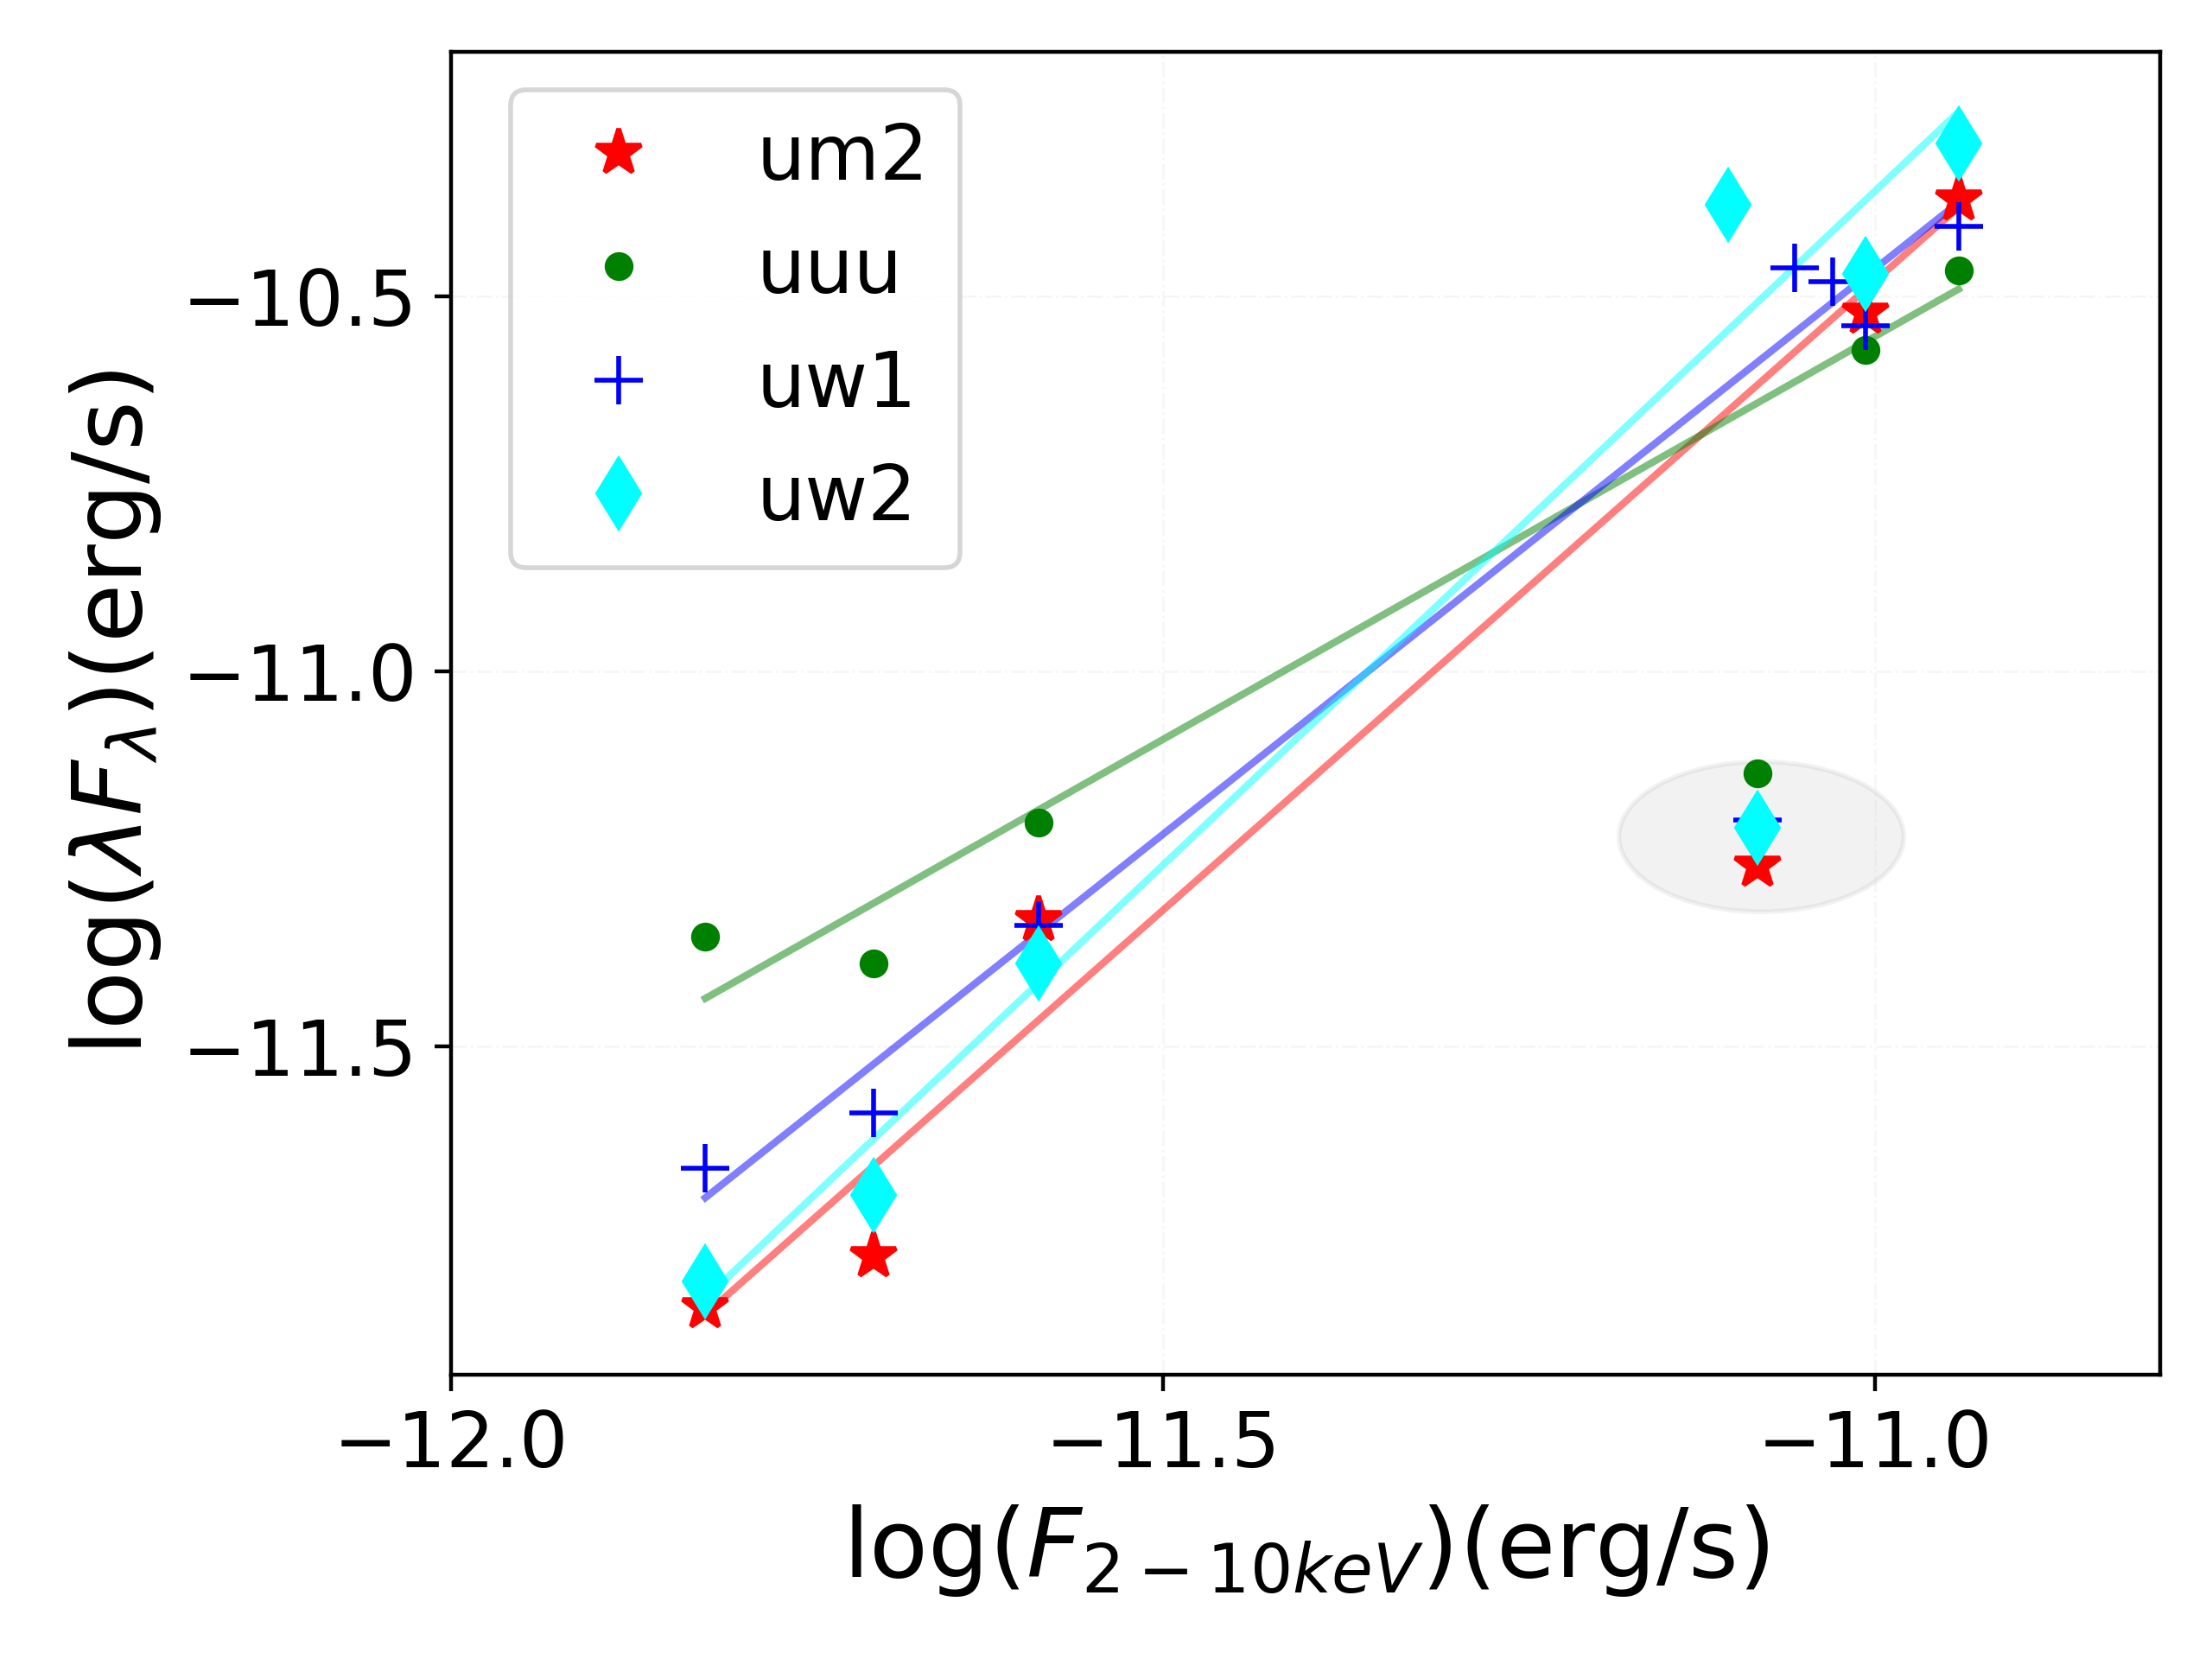
\includegraphics[width=0.9\textwidth]{./pic/uvot_xrt_correlation-fig-without-outlier.png}
    \caption{Correlation of light curve from UVOT and XRT  between 2006 and 2016. Colorful lines represent the linear fit without the outlier in circle.}
    \label{fig:correlation-uvot-xray}
\end{figure*}





\begin{figure*}
\centering
	% To include a figure from a file named example.*
	% Allowable file formats are eps or ps if compiling using latex
	% or pdf, png, jpg if compiling using pdflatex
	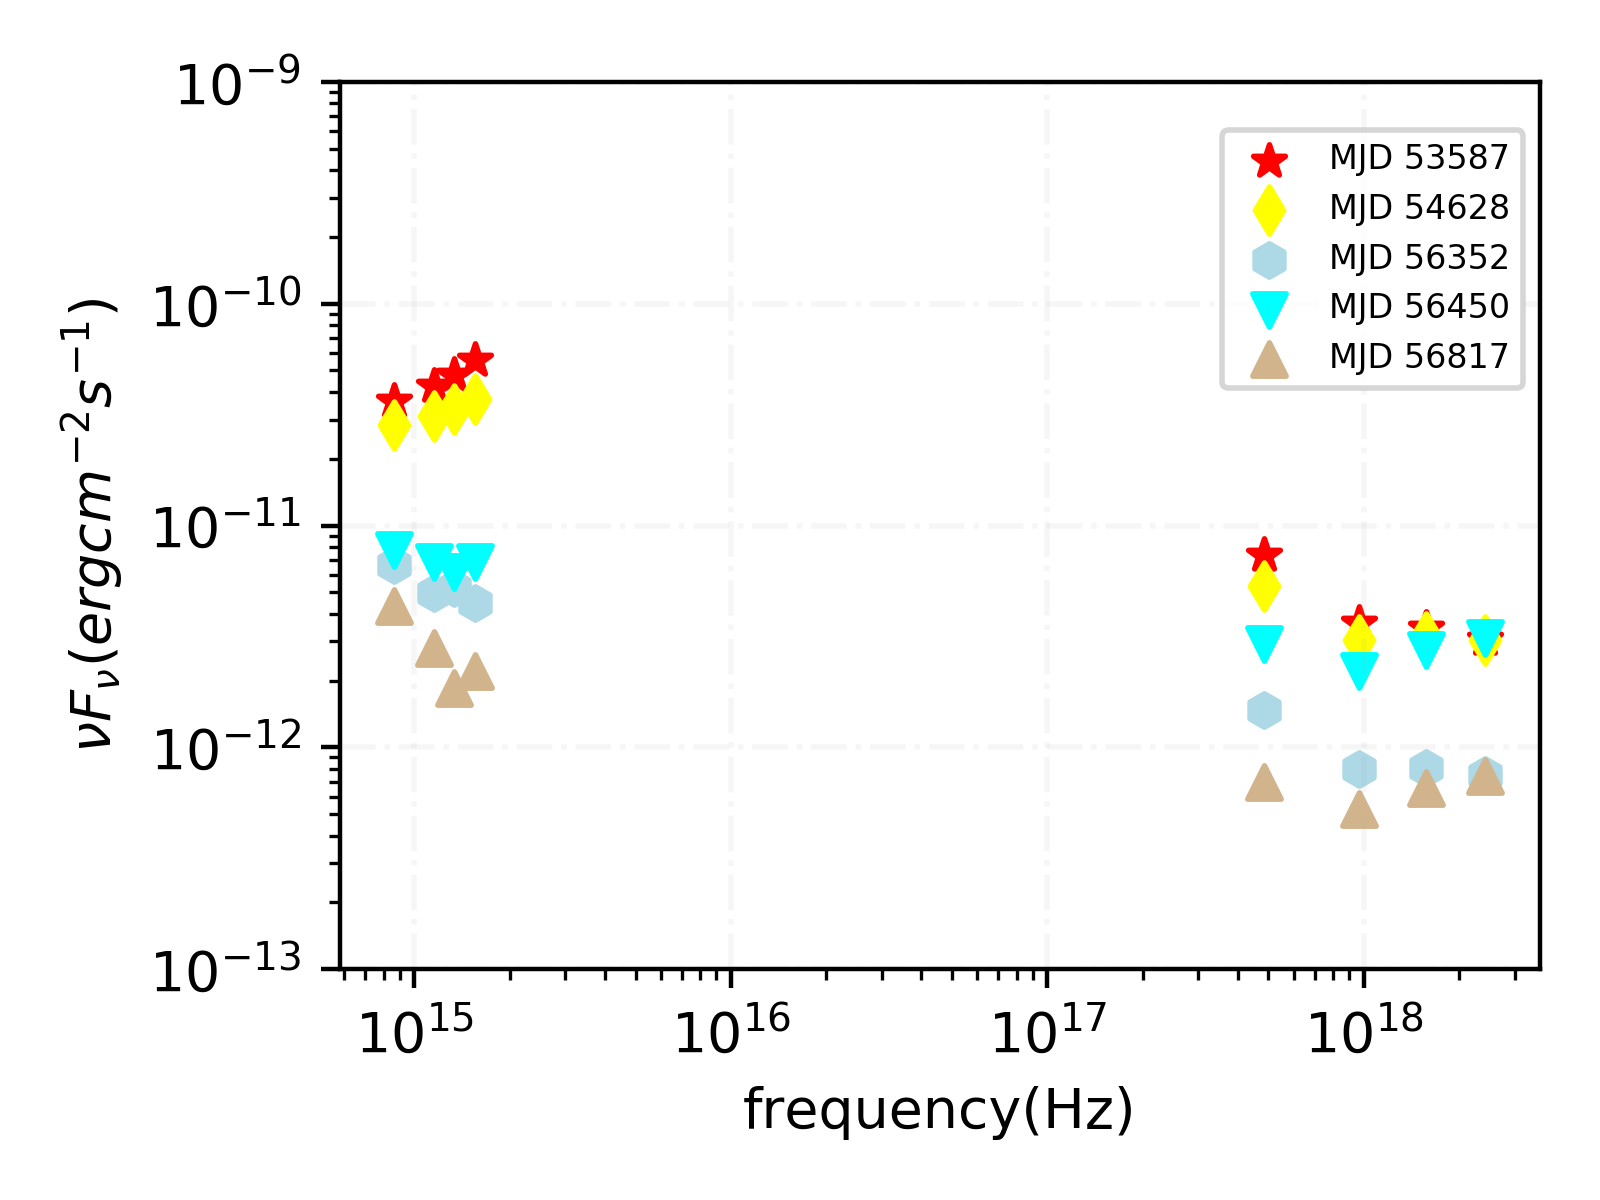
\includegraphics[width=0.9\textwidth]{./pic/Mrk1018_uvot_xray_sed.png}
    \caption{SED between X-ray and ultraviolet}
    \label{fig:xray-uvot-sed}
\end{figure*}

\begin{figure*}
\centering
	% To include a figure from a file named example.*
	% Allowable file formats are eps or ps if compiling using latex
	% or pdf, png, jpg if compiling using pdflatex
	
\includegraphics[width=0.9\textwidth]{./pic/xrayappendgood-errorbar-f-g-tmap.png}
    \caption{$\Gamma$ and flux evolution of Mrk~1018. Blue arrows represent the rapid jump between left and right branches. Grey arrow represents the mini-outburst during 2016-2017.}
    \label{fig:xrayappendgood-fandg-tmap}
\end{figure*}


\begin{figure*}
\centering
	% To include a figure from a file named example.*
	% Allowable file formats are eps or ps if compiling using latex
	% or pdf, png, jpg if compiling using pdflatex
	\includegraphics[width=0.9\textwidth]{./pic/Mrk1018_subplots_alpha_ox_L2vsUV.png}
    \caption{Mrk1018's $\alpha_{OX}-\nu L_{2keV}/L_{Edd}$ and $\alpha_{OX}-\lambda L_{UVW1}/L_{Edd}$ diagram.}
    \label{fig:alpha_ox_luv}
\end{figure*}



\begin{figure*}
\centering
	% To include a figure from a file named example.*
	% Allowable file formats are eps or ps if compiling using latex
	% or pdf, png, jpg if compiling using pdflatex
	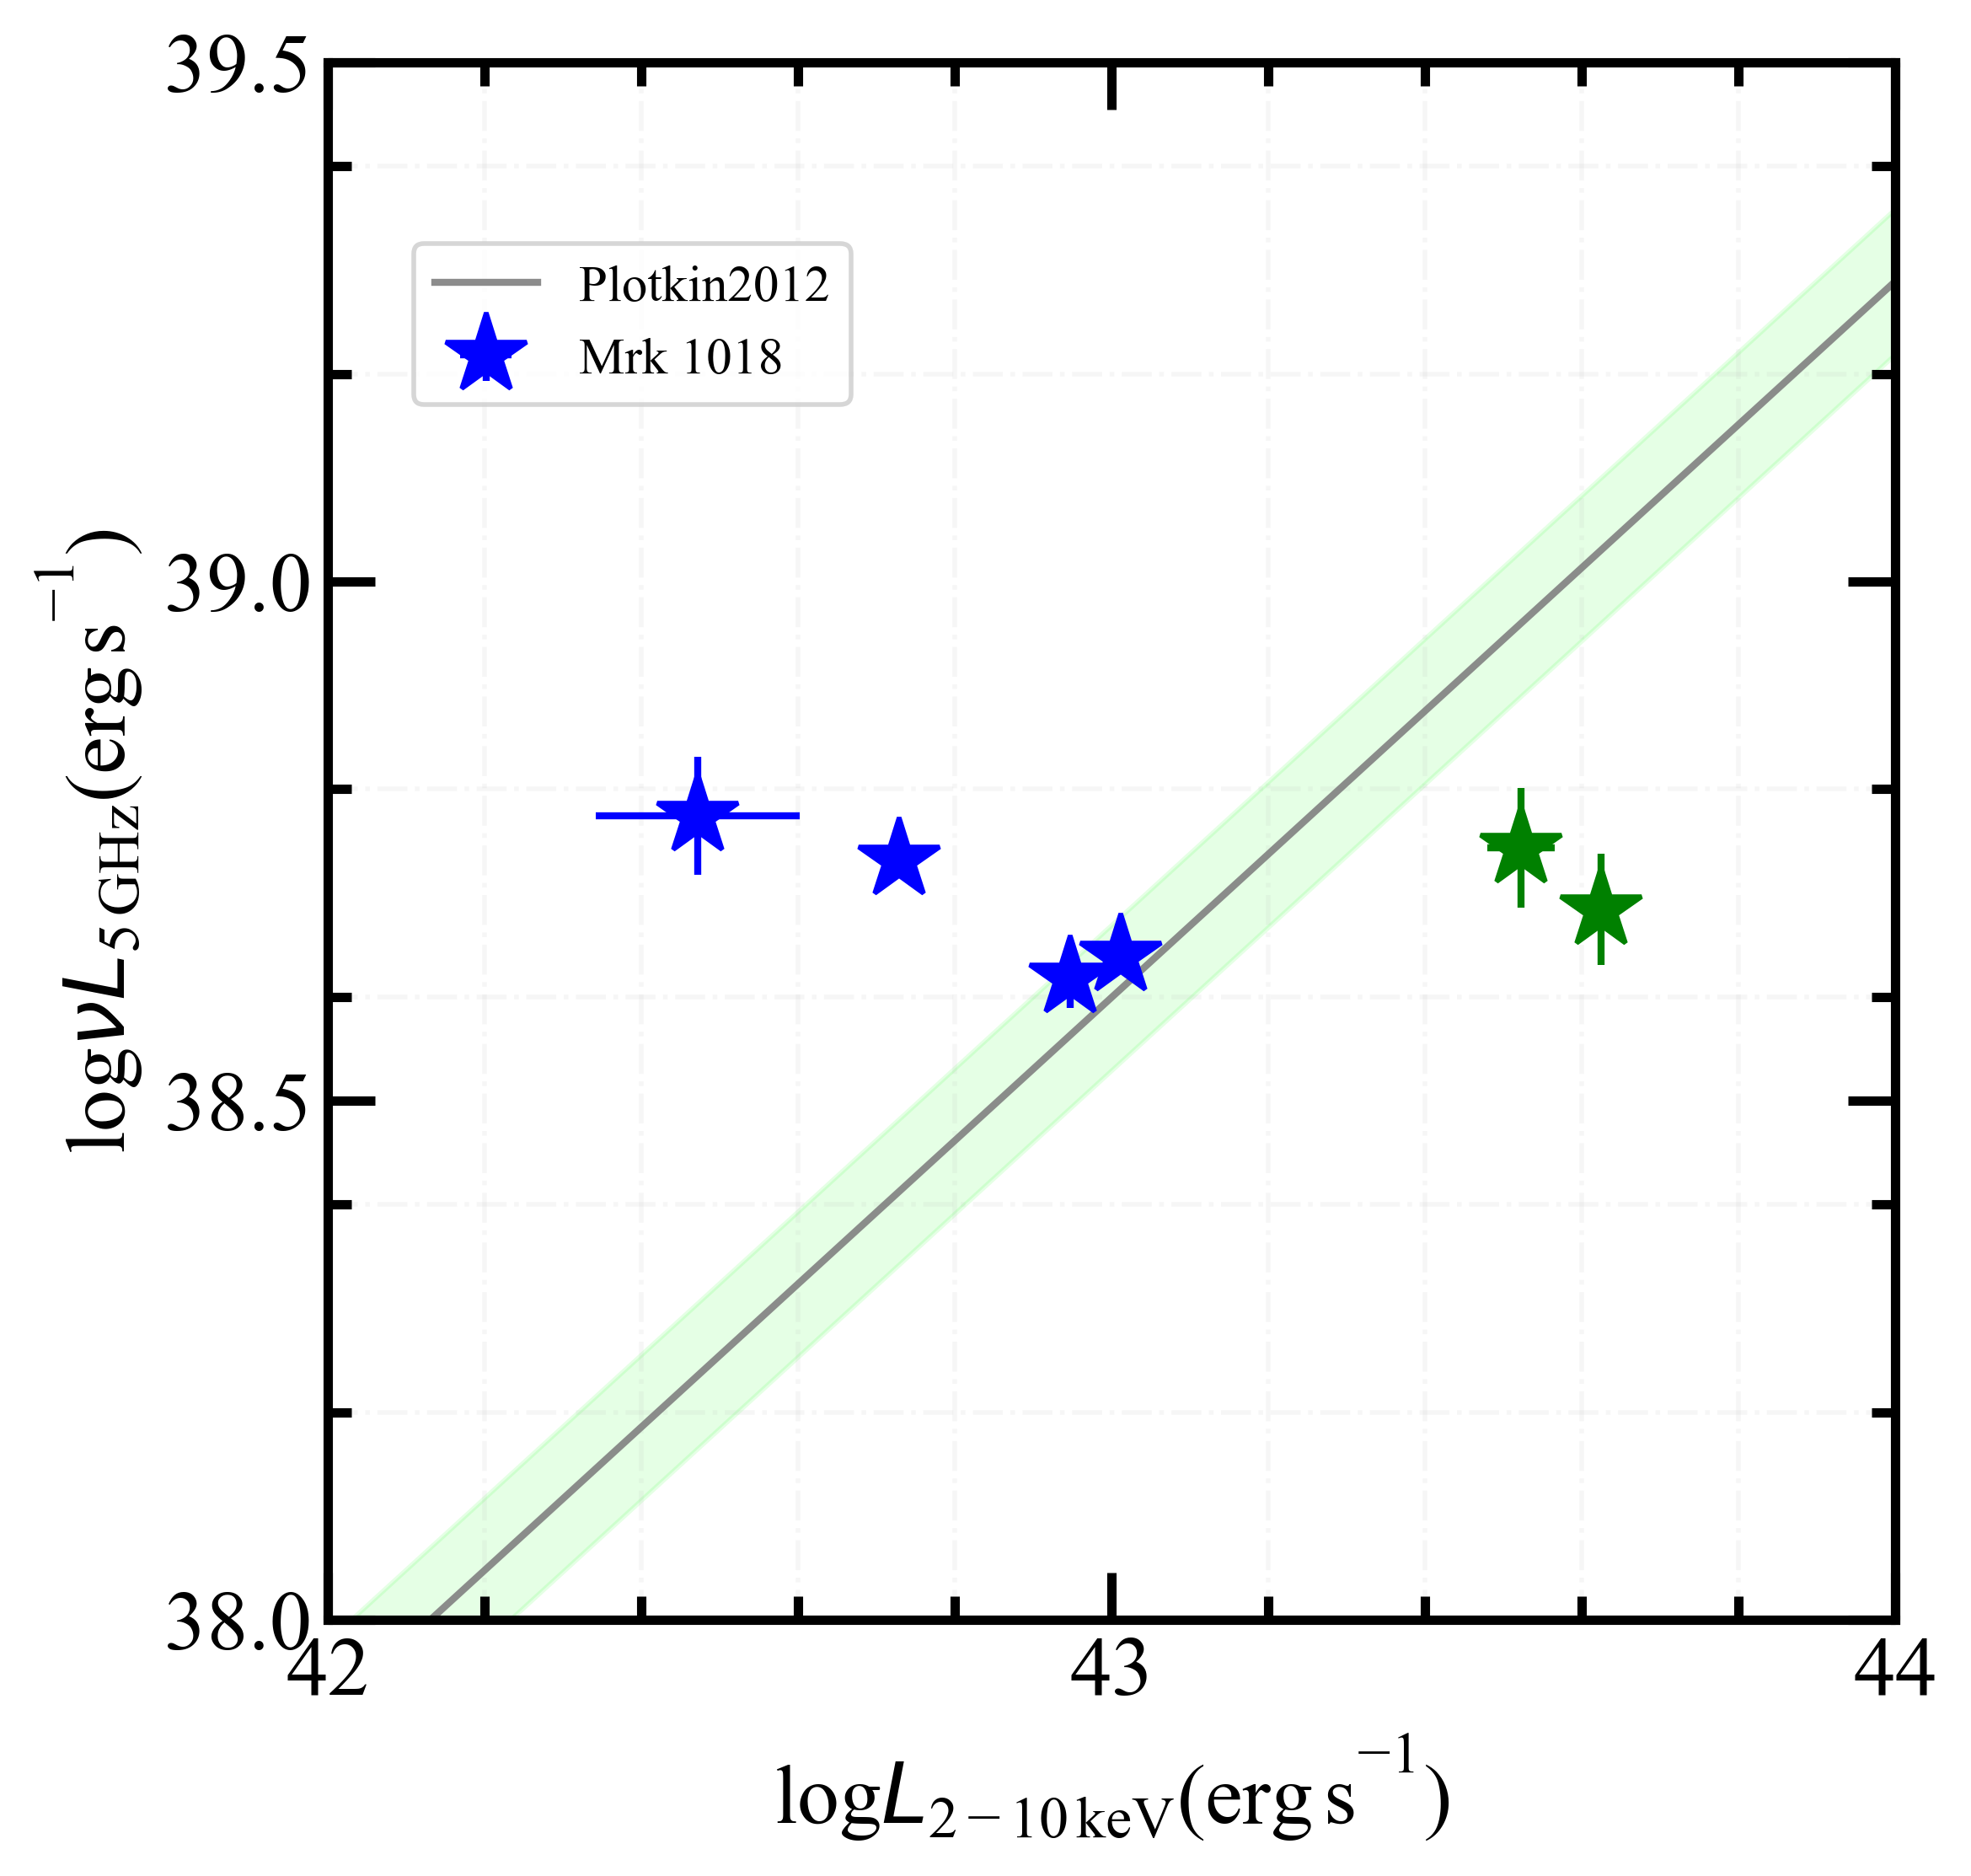
\includegraphics[width=0.9\textwidth]{./pic/Mrk1018_radio_xray_Plotkin2012_Lx.png}
    \caption{Mrk~1018's position in fundamental plane defined in \citet{2012MNRAS.419..267P} (grey straight line) with intrinsic $\sigma=0.07$, where shallow vertical region shows the critical luminosity between lower flux(4$\times$ 10$^{-12}$ erg cm$^{-2} $s$^{-1}$) and upper flux (7$\times$ 10$^{-12}$ erg cm$^{-2}$ s$^{-1}$).}
    \label{fig:radio-xray-mass_relation_Plotkin2012}
\end{figure*}


%% We thank Linhui Wu for disscussion on the VLA data reduction. This work is supported by...
%% To help institutions obtain information on the effectiveness of their 
%% telescopes the AAS Journals has created a group of keywords for telescope 
%% facilities.
%
%% Following the acknowledgments section, use the following syntax and the
%% \facility{} or \facilities{} macros to list the keywords of facilities used 
%% in the research for the paper.  Each keyword is check against the master 
%% list during copy editing.  Individual instruments can be provided in 
%% parentheses, after the keyword, but they are not verified.




%% Appendix material should be preceded with a single \appendix command.
%% There should be a \section command for each appendix. Mark appendix
%% subsections with the same markup you use in the main body of the paper.

%% Each Appendix (indicated with \section) will be lettered A, B, C, etc.
%% The equation counter will reset when it encounters the \appendix
%% command and will number appendix equations (A1), (A2), etc. The
%% Figure and Table counter will not reset.

\clearpage
%\bibliographystyle{mnras}
\bibliography{refMrk1018}{}
% if your bibtex file is called example.bib
\bibliographystyle{aasjournal}
%\clearpage

\begin{table}
\centering
\caption{{ \bf X-ray fit parameters of Mrk~1018. } Columns include the date of the observation, the facility, observation id, reduced $\chi ^2$ of the best fit model, the photon index $\Gamma$ with 90\% uncertainty, and the flux in 2-10~keV after Galactic-absorption correction. }
\label{tab:table1}

\begin{tabular}{lcccccc}
\hline
\hline
 
  Date   &   Instrument & obsid  & $\chi ^2$  &$\Gamma$  &  $F_{2-10keV}$  & \\ 
  (MJD)  &              &        &          &                    &  [erg cm$^{-2}$ s$^{-1}$] &      
 \\  \hline
53385 & X & 201090201 & 0.98 & 1.73 $\pm$ 0.07 & 9.7e-12 $\pm$ 6e-13 \\ 
53587 & S & 35166001 & 0.78 & 1.93 $\pm$ 0.1 & 1.15e-11 $\pm$ 6.99e-13 \\ 
54271 & S & 30955001 & 1.01 & 1.89 $\pm$ 0.09 & 9.39e-12 $\pm$ 4.47e-13 \\ 
54274 & S & 30955002 & 1.07 & 1.91 $\pm$ 0.08 & 8.54e-12 $\pm$ 4e-13 \\ 
54276 & S & 30955003 & 1.02 & 1.96 $\pm$ 0.08 & 8.38e-12 $\pm$ 3.47e-13 \\ 
54628 & S & 35776001 & 1.19 & 1.75 $\pm$ 0.07 & 9.98e-12 $\pm$ 3.96e-13 \\ 
54685 & X & 554920301 & 1.16 & 1.79 $\pm$ 0.02 & 1.13e-11 $\pm$ 2e-13 \\ 
55527$^{(a)}$ & C & 12868 & 1.1 & 1.7 $\pm$ 0.03 & 9.26e-12 $\pm$ 1.9e-13 \\ 
56353 & S & 49654001 & 1.42 & 1.82 $\pm$ 0.38 & 2.59e-12 $\pm$ 5.52e-13 \\ 
56450 & S & 49654002 & 1.23 & 1.38 $\pm$ 0.19 & 7.9e-12 $\pm$ 8.21e-13 \\ 
56818 & S & 49654004 & 0.75 & 1.38 $\pm$ 0.31 & 1.88e-12 $\pm$ 3.37e-13 \\ 
57428 & N & 60160087002 & 1.23 & 1.85 $\pm$ 0.08 & 1.8e-12 $\pm$ 1e-13 \\ 
57429 & S & 80898001 & 0.96 & 1.72 $\pm$ 0.2 & 1.61e-12 $\pm$ 1.89e-13 \\ 
57434 & S & 80898002 & 0.9 & 1.45 $\pm$ 0.2 & 2.17e-12 $\pm$ 2.77e-13 \\ 
57443 & C & 18789 & 0.82 & 1.7 $\pm$ 0.03 & 1.3e-12 $\pm$ 3e-14 \\ 
57801 & C & 19560 & 1.26 & 1.61 $\pm$ 0.02 & 2.48e-12 $\pm$ 4e-14 \\ 
58123 & N & 60301022002 & 1.34 & 1.8 $\pm$ 0.06 & 2.1e-12 $\pm$ 1e-13 \\ 
58125 & S & 88207001 & 1.04 & 1.63 $\pm$ 0.25 & 2.02e-12 $\pm$ 3.08e-13 \\ 
58126 & C & 20366 & 1.05 & 1.6 $\pm$ 0.03 & 1.84e-12 $\pm$ 5e-14 \\ 
58180 & C & 20367 & 1.02 & 1.61 $\pm$ 0.04 & 1.59e-12 $\pm$ 5e-14 \\ 
58182 & N & 60301022003 & 1.03 & 1.8 $\pm$ 0.06 & 1.5e-12 $\pm$ 7e-14 \\ 
58281 & C & 20368 & 1.02 & 1.62 $\pm$ 0.03 & 1.77e-12 $\pm$ 5e-14 \\ 
58316 & N & 60301022005 & 0.85 & 1.74 $\pm$ 0.05 & 2e-12 $\pm$ 9e-14 \\ 
58317 & S & 88207003 & 1.01 & 1.61 $\pm$ 0.23 & 2.18e-12 $\pm$ 3.12e-13 \\  \\ \hline
\end{tabular}\\
Notes: Here the superscripts $^{(a)}$ represents fit result that are taken from \citet{2017A&A...607L...9K}. Instrument indicate by C-\chandra, S-\swift, X-\xmm, N-\nustar. 
\end{table}
\clearpage







\begin{table}
\centering
\caption{{\bf $\alpha_{ox}$ of Mrk~1018 with simultaneous XRT and UVOT observation.} Columns include the date of the observation, $\alpha_{ox}$, flux in 2-10~keV, $\nu F_{uw1}$, and Eddington rate.}
\label{tab:tablealpha_ox}
\begin{tabular}{lcccccc}
\hline
\hline
 
 Date &   $\alpha_{ox}$  & $F_{2-10keV}$  &$\nu F_{uw1}$  & $L_{2-10keV}/L_{Edd}$ &   $\nu L_{uw1}/L_{Edd}$  \\ 
 (MJD)&                   &   [erg cm$^{-2}$ s$^{-1}$]   &[erg cm$^{-2}$ s$^{-1}$]    &                    &            
 \\ \hline
53587 & 1.29 & 1.14e-11 & 3.92e-11 & 5.53e-03 & 1.90e-02 \\ 
54271 & 1.30 & 9.34e-12 & 3.31e-11 & 4.51e-03 & 1.60e-02 \\ 
54275 & 1.31 & 8.78e-12 & 3.45e-11 & 4.24e-03 & 1.67e-02 \\ 
54628 & 1.29 & 9.85e-12 & 2.89e-11 & 4.76e-03 & 1.40e-02 \\ 
56352 & 1.20 & 2.59e-12 & 4.58e-12 & 1.25e-03 & 2.22e-03 \\ 
56450 & 1.14 & 8.26e-12 & 6.35e-12 & 3.99e-03 & 3.07e-03 \\ 
56817 & 1.23 & 1.98e-12 & 2.58e-12 & 9.57e-04 & 1.25e-03 \\ \hline
\end{tabular}   
\end{table}
\begin{table}
\centering
\caption{{\bf VLA observation of Mrk~1018.} Columns include the date of observation, project name, band, frequency, integrated flux, radio spectral index ($\alpha$) and reference.}
\label{tab:tableradio}
\begin{tabular}{lcccccr}
\hline
\hline
 
 Date &  project & band  & Frequency  &$F_{int}$   & $\alpha$ & Reference  \\ 
 (MJD)&         &        &   [GHz]   &[mJy]     &                &         \\ \hline
    \multirow{2}*{46032} & \multirow{2}*{AU0020} & L    & 1.49  & 4.21  $\pm$ 0.23  & \multirow{2}*{0.52 $\pm0.07$} &\\
    \,          &        & C     & 4.86  & 2.29  $\pm$ 0.14  & & \\
    47261     & AB0476 & C     & 4.86  & 1.91  $\pm$ 0.23  &  &\\
    47692     & AB0540A & C     & 4.86  & 2.62  $\pm$ 0.16  &  &\\
    47732     & AB0540B & C     & 4.86  & 2.31  $\pm$ 0.17  & & \\
    49820.5 $\pm$ 773.5 & AB0628 & L     & 1.4   & 4.20  $\pm$ 0.45  &  & \citet{1998AJ....115.1693C} \\
    49820.5 $\pm$ 773.5 & AB0628 & L     & 1.4   & 4.15  $\pm$ 0.25  &  & \citet{1997ApJ...475..479W} \\
    50219.5 $\pm$ 1078.5 & AB0308 & L     & 1.4   & 4.20  $\pm$ 0.54  &  & \citet{2002AJ....124..675C}\\
    50970     & AB0878 & X     & 8.46  & 2.47  $\pm$ 0.17  & 0.3 $\pm0.08$\\
    52246.5 $\pm$ 278.5 & AB0950 & L     & 1.4   & 4.15  $\pm$ 0.25  & & \citet{2003yCat.8071....0B} \\
    54872.5 $\pm$ 51.5  & AR685 & L     & 1.4   & 3.69  $\pm$ 0.19  &  & \citet{2011AJ....142....3H}\\
    54878   & AB1314 & L     & 1.4   & 3.36  $\pm$ 0.20  &  & \citet{2012yCat.8090....0B} \\
    56550 $\pm$ 8     & 13B-272 & L     & 1.4   & 3.85  $\pm$ 0.31  &  & \citet{2016MNRAS.460.4433H} \\

    \multirow{3}*{57481}     &  \multirow{3}*{16A-444} & C     & 5     & 2.56  $\pm$ 0.13  & \multirow{3}*{0.02$\pm0.05$}& \\
              &     & X     & 10    & 2.16  $\pm$ 0.11  & &\\
              &    &  K     & 22    & 2.46  $\pm$ 0.12  &  &\\
    57719     & 16B-084 & X     & 10    & 1.78  $\pm$ 0.09  &   &\\

    57731     & 16B-084 & X     & 10    & 1.97  $\pm$ 0.10  &  &\\

    57768     & 16B-084 & C     & 5     & 2.07  $\pm$ 0.10  & 0 &\\
    58087     & VLASS1.1 & L     & 3     & 2.30  $\pm$ 0.36  & & \\
    
    58472     & 18B-245 & K     & 20    & 2.71  $\pm$ 0.14  &  & \\



\hline 
\end{tabular}   
\end{table}




     
\begin{table}
\centering
\caption{{\bf Radio and X-ray luminosity diagram.} Columns include the date of the radio observation, the radio spectrum index $\alpha_{radio}$, the date of X-ray observation, the interval between two bands, the flux and luminosity rescaled to 4.8 and 8.4~GHz, the X-ray flux and luminosity in 2-10~keV band.}
\label{tab:table4}
\begin{tabular}{lllllllllr}
\hline
\hline

$T_{Radio}$ &  $\alpha_{Radio}$ & $T_{X-ray}$ & $\delta$ T & $F_{2-10keV}$ & $F_{4.8GHz}$ & $F_{8.4GHz}$ &  $\nu L_{\nu=4.8GHz}$ &  $\nu L_{\nu=8.4GHz}$ & $L_{\rm{2--10~keV}}$ \\ 
(MJD)  &  & (MJD)  &(day)  &[erg$~s^{-1}~\rm{cm}^{-2}$] & [mJy)& (mJy)]& [erg$~s^{-1} $] & [erg$~s^{-1} $]& [erg$~s^{-1} $]\\
\hline

52246.5 & 0.42 & 53385 & 1138 & 9.70e-12 & 2.47 & 1.96 & 5.00e38 & 6.92e38 & 4.09e43 \\ 
54318 & 0.42 & 54276 & 42 & 8.78e-12 & 2.00 & 1.58 & 4.05e38 & 5.60e38 & 3.70e43 \\ 
54872.5 & 0.42 & 54685 & 188 & 1.13e-11 & 2.20 & 1.74 & 4.45e39 & 6.15e39 & 4.76e44 \\ 
56550 & 0.42 & 56450 & 100 & 8.26e-12 & 2.29 & 1.81 & 4.64e40 & 6.42e40 & 3.48e45 \\ 
57481 & 0.17 & 57443 & 38 & 1.30e-12 & 2.49 & 2.27 & 5.04e41 & 8.02e41 & 5.48e45 \\ 
57768 & 0.17 & 57801 & 33 & 2.48e-12 & 2.00 & 1.82 & 4.05e42 & 6.45e42 & 1.04e47 \\  \hline
\end{tabular}\\
Notes: We assume the $\alpha_{Radio}$ before/after the type transition as a constant, respectively. 
\end{table}


%\appendix
%\section{Appendix}


%\clearpage


%\clearpage


%% For this sample we use BibTeX plus aasjournals.bst to generate the
%% the bibliography. The sample63.bib file was populated from ADS. To
%% get the citations to show in the compiled file do the following:
%%
%% pdflatex sample63.tex
%% bibtext sample63
%% pdflatex sample63.tex
%% pdflatex sample63.tex




%% This command is needed to show the entire author+affiliation list when
%% the collaboration and author truncation commands are used.  It has to
%% go at the end of the manuscript.
%\allauthors

%% Include this line if you are using the \added, \replaced, \deleted
%% commands to see a summary list of all changes at the end of the article.
%\listofchanges
% Don't change these lines
%\bsp	% typesetting comment
%\label{lastpage}
\end{document}

% End of file `sample63.tex'.
